\documentclass[11pt,a4paper]{article}

% ===== Packages =====
\usepackage[utf8]{inputenc}
\usepackage[T1]{fontenc}
\usepackage{newtxtext,newtxmath}
\usepackage[margin=1in]{geometry}
\usepackage{graphicx}
\usepackage{booktabs}
\usepackage{cite}
\usepackage{array}
\usepackage{hyperref}
\usepackage{xcolor}
\usepackage{amssymb}
\usepackage{enumitem}
\usepackage{subcaption}
\usepackage{makecell}
\usepackage{tabularx}
\usepackage{float}
\usepackage{fancyhdr}
\usepackage{titlesec}
\usepackage{titling}
\usepackage{amsmath}
\usepackage{parskip}
\usepackage[htt]{hyphenat}
\usepackage{listings}
\usepackage{tikz}
\usetikzlibrary{arrows.meta, positioning, shapes.geometric}
\usepackage{mdframed}
\usepackage{algorithm}
\usepackage{algpseudocode}
\usepackage{xurl}
% \pdfobjcompresslevel=0
% ===== Listings style for code =====
\lstset{
  basicstyle=\ttfamily\small,
  keywordstyle=\color{blue!70!black}\bfseries,
  commentstyle=\color{green!50!black},
  stringstyle=\color{red!60!black},
  breaklines=true,
  frame=single,
  framerule=0.4pt,
  rulecolor=\color{black!30},
  backgroundcolor=\color{black!3},
  xleftmargin=1em,
  framexleftmargin=0.5em,
  language=Python,
  showstringspaces=false
}

% ===== Styling =====
\definecolor{titleRed}{RGB}{170,30,45}

\hypersetup{
    colorlinks=true,
    linkcolor=blue!70!black,
    citecolor=blue!70!black,
    urlcolor=blue!70!black
}

\pagestyle{fancy}
\fancyhf{}
\fancyhead[L]{\small\sffamily\color{titleRed} OMC: Running Self-Evolving Agent Teams on Arbitrary Tasks Like a Real-World Company}
\fancyhead[R]{\small\sffamily\color{black!50} \thepage}
\renewcommand{\headrulewidth}{0.4pt}

\titleformat{\section}{\Large\bfseries}{\thesection}{0.5em}{}
\titleformat{\subsection}{\large\bfseries}{\thesubsection}{0.5em}{}
\titleformat{\subsubsection}{\normalsize\bfseries}{\thesubsubsection}{0.5em}{}
\setlength{\droptitle}{-4.5em}

% ===== Title =====

\title{\bfseries\color{titleRed}
OneManCompany:\\[6pt]
Running Self-Evolving Agent Teams on Arbitrary Tasks Like a Real-World Company
}
\vspace{-3.2cm}

\author{
\textbf{Zhengxu Yu}$^{1,*,\dagger}$,
\textbf{Yu Fu}$^{1,*}$,
\textbf{Zhiyuan He}$^{1}$,
\textbf{Yuxuan Huang}$^{3}$,
\textbf{Lee Ka Yiu}$^{1}$,\\
\textbf{Meng Fang}$^{3}$,
\textbf{Weilin Luo}$^{1}$,
\textbf{Jun Wang}$^{2}$
}
\renewcommand{\thefootnote}{}
\footnotetext{\hspace{-1.8em}%
\begin{minipage}[t]{\textwidth}
\raggedright
$^{1}$HUAWEI Noah's Ark Lab \,\,
$^{2}$University College London \,\,
$^{3}$University Liverpool \\
$^{*}$Co-first author \,\,
\quad $^{\dagger}$Corresponding Author: \texttt{\{zhengxu.yu\}@h-partners.com}
\end{minipage}
}
\renewcommand{\thefootnote}{\arabic{footnote}}
 
\date{}

\begin{document}
\vspace{-3.2cm}
\maketitle
\thispagestyle{empty}
\vspace{-1.6em}

\begin{center}
Project Homepage: \url{https://1mancompany.github.io/OneManCompany/} \\
Repository: \url{https://github.com/1mancompany/OneManCompany}
\end{center}

\begin{abstract}
Current multi-agent frameworks either hardcode team structures or constrain all agents to a single runtime, limiting them to pre-configured workflows.  Real projects demand what we call \emph{wild dynamic agentic workflows}: the team, the task decomposition, and even the agent backends may all need to change mid-execution.  We present OneManCompany (OMC), an open-source framework that organises heterogeneous AI agents the way a human company organises its employees.  Like an operating system for a virtual company, OMC separates each AI employee into a portable identity (Talent) and an execution runtime (Vessel), connected through a typed Harness that manages scheduling, communication, and lifecycle.  On top of this, OMC introduces an Explore-Execute-Review tree search algorithm for wild workflow coordination, paired with DAG-based task decomposition that provides formal guarantees on termination and deadlock freedom.  Deep integration with a community-driven Talent Market (\url{one-man-company.com}) supplies verified agents on demand, since new capabilities can be recruited mid-project rather than pre-configured at design time.  Agents and the organisation itself self-evolve through structured retrospectives, CEO one-on-ones, and a formal performance review pipeline.  On PRDBench, a project-level software development benchmark, OMC achieves an 84.67\% success rate, surpassing all baselines.  We further demonstrate OMC's cross-domain generality through case studies spanning multiple industries.
\end{abstract}

\begin{figure}[H]
    \centering
    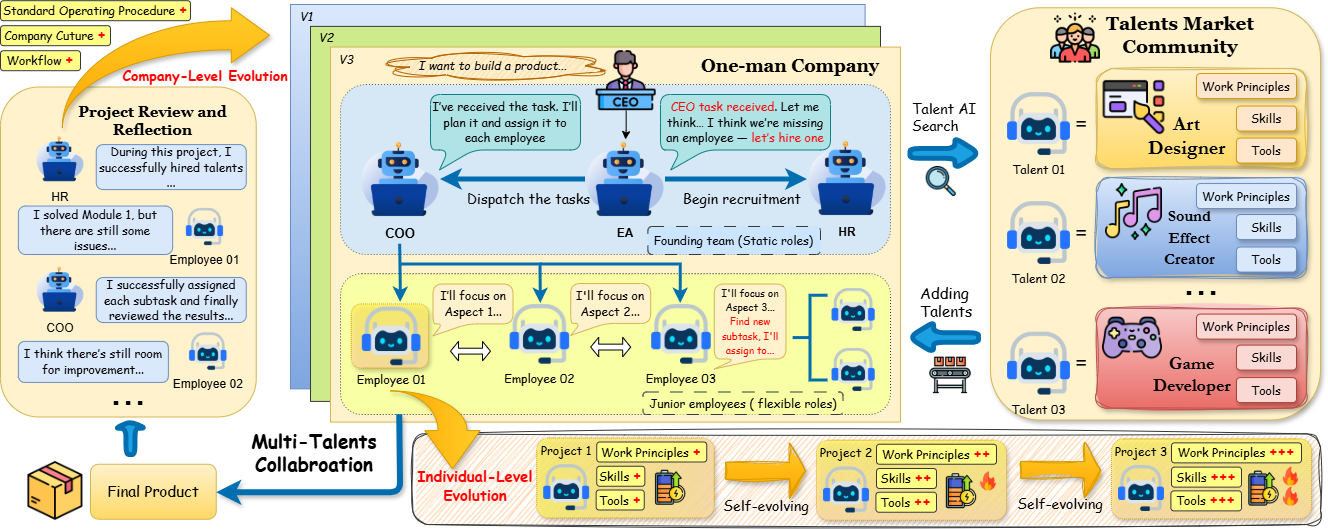
\includegraphics[width=0.9\textwidth]{oneman-com2.png}
    \caption{
\textbf{Overview of the OMC system.} The central hierarchy mirrors a real company: tasks flow from the CEO or external clients to downstream AI talents. Agents collaborate in a tree-like structure reflecting organizational workflows. The Talent Market (right) allows HR to recruit specialized agents on demand. Individual-Level Evolution (bottom) enables agents to self-improve through tasks, while Project Review (left) supports collective reflection and drives Company-Level Evolution.
}
    \label{fig:overview}
\end{figure}

\clearpage

% =====================================================================
\section{Introduction}
\label{sec:introduction}
% =====================================================================

Individual AI agents such as Claude Code~\cite{anthropic2024claudecode}, Codex~\cite{openai2024codex}, and OpenClaw~\cite{openclaw2024} can now write code, search the web, generate images, and reason about complex tasks.  But what happens when a project requires more than one agent?  Building a product, conducting a research study, or producing multimedia content demands a \emph{team}: someone to plan, someone to execute, someone to review, and often specialists that need to be recruited mid-project.  Today, orchestrating such a team falls entirely on the user.  Few existing frameworks address the question: \textbf{how should these agents be organized?}

Human companies have been answering a version of this question for centuries.  A startup, a film studio, and a law firm all look different on the surface, but they share the same organizational machinery: manage a workforce under uniform policies, decompose projects into tasks with clear ownership, hire specialists when capabilities are missing, and learn from retrospectives to do better next time.  The machinery is industry-agnostic because it is decoupled from what individual employees actually know.  We argue that the same decoupling could apply to AI agent workforces.

Current multi-agent frameworks fall short of this vision.  Recent work on \emph{dynamic agentic workflows}~\cite{wang2025tdag, erdogan2025planact, hu2025evomac} has shown that adapting task decomposition at runtime outperforms static pipelines.  But even these systems operate within a pre-configured sandbox: the team is fixed before the project starts, all agents share the same runtime, and the workflow topology is constrained to a known template.  What real projects demand are \emph{wild dynamic agentic workflows}, i.e., workflows where none of the four key dimensions (team composition, task decomposition, agent runtime, agent capabilities) is fixed before execution.  A user should be able to hand an arbitrary one-sentence project brief to the system and walk away, regardless of domain.

Existing frameworks offer limited support for this.  LangChain~\cite{langchain2024deepagents}, CrewAI, AutoGen, and Paperclip~\cite{paperclip2025} either hardcode team structures (brittle to novel projects) or let agents negotiate freely (no convergence guarantees).  Agents from different families cannot interoperate because they are locked into incompatible runtimes.  Roles are specified through descriptive prompts rather than executable contracts, leading to hallucinated capabilities.  And self-improvement, where it exists, is session-bound and framework-specific.  What is missing is an organizational layer, analogous in function to an operating system but for agent workforces, that abstracts over runtimes, manages lifecycles, and enforces coordination invariants while leaving everything else unconstrained.

We introduce OneManCompany (OMC), an open-source multi-agent framework that fills this gap.  OMC is built on four components (Figure~\ref{fig:overview}):

\begin{enumerate}[nosep]
\item \textbf{Harness Engineering} (Section~\ref{sec:harness}).  A typed Talent\,--\,Vessel\,--\,Harness architecture that separates \emph{who an agent is} (the Talent: prompts, skills, tools) from \emph{where it runs} (the Vessel: LangGraph, Claude CLI, or script process).  Six typed interfaces mediate all agent--platform interaction, so adding a new runtime does not require changes to scheduling or lifecycle logic.

\item \textbf{Explore-Execute-Review Tree Search and DAG-based Task Decomposition} (Sections~\ref{sec:explore-review} and~\ref{sec:dag}).  OMC models project execution as a search over organizational strategies.  The system explores decomposition options, expands the task tree, executes work through agents, and reviews results to refine future decisions.  An AND-tree with a finite state machine provides formal guarantees on termination, deadlock freedom, and crash recovery.

\item \textbf{Talent Market} (Section~\ref{sec:talent-market}).  When a project requires capabilities that the current team lacks, OMC recruits from a community-driven marketplace\,\footnote{\url{https://one-man-company.com/}} of verified agent implementations.  Agents are grounded in executable, tested artefacts rather than descriptive prompts, so their capabilities are what they claim to be.

\item \textbf{Self-Evolution} (Section~\ref{sec:self-evolution}).  Agents refine their working principles through CEO one-on-ones and post-task reflection.  Project retrospectives distil lessons into updated SOPs.  A formal performance review pipeline (periodic evaluations, Performance Improvement Plans, and automated offboarding) creates real consequences, the same way human HR does.
\end{enumerate}

On PRDBench, a project-level software development benchmark, OMC achieves an 84.67\% success rate, surpassing all baselines.

\section{Related Work}
\label{sec:related}

OMC draws on ideas from several lines of research: multi-agent frameworks and their approaches to heterogeneity, agent marketplaces and tool integration protocols, task planning and workflow execution, team composition and organisational hierarchy, and mechanisms for agent self-improvement.  We review each in turn.

\subsection{LLM-Based Multi-Agent Frameworks}
\label{sec:rw-mas}

Recent multi-agent systems have moved toward heterogeneous, dynamically composed teams. Magentic-One~\cite{fourney2024magenticone} and OWL~\cite{hu2025owl} use specialised orchestrators and hierarchies; X-MAS~\cite{ye2025xmas} and MacNet~\cite{qian2025macnet} show that heterogeneous DAG topologies outperform homogeneous baselines. Other lines of work explore RL-based orchestration~\cite{dang2025evolving}, structured memory~\cite{yuen2025intrinsic}, and OS-level management~\cite{agentforge2025, wang2025openhands, mei2025aios}. However, heterogeneity in these frameworks is limited to the model level: all agents still share the same execution runtime. OMC goes further: the Vessel\,+\,Talent abstraction decouples execution containers from capabilities, so a single dispatch loop can orchestrate LangChain agents, Claude~CLI sessions, and script-based processes side by side.


\subsection{Agent Marketplaces and Tool Integration}
\label{sec:rw-ecosystem}

Protocols like MCP~\cite{hou2025mcp} and A2A~\cite{google2025a2a} standardise tool integration and inter-agent communication, while decentralised agent registries are emerging~\cite{singh2025registry, ehtesham2025interop}. Platforms such as Cerebrum~\cite{rama2025cerebrum, mei2025aios}, AgentStore~\cite{jia2025agentstore}, OpenHands~\cite{wang2025openhands}, and AgentScope~\cite{gao2025agentscope} host community-contributed agents and tool catalogues~\cite{yang2025sweagent, mcpzoo2025}. These ecosystems handle tool-level composition well, but none offers a marketplace where complete agent packages (skills, tools, scripts, and persona) can be discovered, interviewed, and onboarded into a persistent organisation. OMC's Talent Market fills this gap: the HR agent queries the marketplace, the CEO interviews candidates, and an automated pipeline provisions the selected agent end-to-end.


\subsection{Task Planning and Workflow Execution}
\label{sec:rw-workflow}

A growing body of work adapts task decomposition at runtime rather than planning everything upfront~\cite{wang2025tdag, erdogan2025planact, paglieri2025learnplan}, and several systems evolve workflow topologies through code search~\cite{zhang2025aflow} or test-time self-evolution~\cite{hu2025evomac}; recent surveys catalogue this shift~\cite{yu2025workflowsurvey, huang2025plansurvey}. Existing platforms manage tasks via ticket-based inheritance~\cite{paperclip2025}, pipeline abstractions~\cite{gao2025agentscope}, or hierarchical sub-goal formulation~\cite{agentorchestra2025}, but they typically cannot expand the task tree at runtime. OMC's task tree grows during execution: subtasks are created on the fly with explicit dependency tracking, results are validated before propagating downstream, failed tasks are retried with a circuit breaker that escalates to the CEO after repeated failures, and asynchronous external events (e.g., human feedback) are handled via dedicated pause states.


\subsection{Team Composition and Organisational Design}
\label{sec:rw-org}

Multi-agent team composition ranges from fully fixed to fully dynamic. On the dynamic end, DyLAN~\cite{liu2025dylan}, AFlow~\cite{zhang2025aflow}, AgentSquare~\cite{shang2025agentsquare}, and EvoMAC~\cite{hu2025evomac} assemble teams on the fly using scoring, search, or self-evolution; scaling-law studies suggest compact core teams work best~\cite{qian2025macnet, tran2025masurvey}. On the fixed end, orchestrator-worker hierarchies~\cite{fourney2024magenticone, hu2025owl}, sub-goal allocators~\cite{agentorchestra2025}, and council models~\cite{teamofrivals2025} pre-define structure. Paperclip~\cite{paperclip2025} puts the human in a strategic director role but provides no founding team to bootstrap from. OMC takes a hybrid approach: a founding C-suite (EA, HR, COO, CSO) is always present to handle cold start and routine coordination, while the human CEO recruits and dismisses domain specialists as projects require.

\subsection{Self-Improving and Self-Evolving Agents}
\label{sec:rw-selfevo}

At the individual level, agents can now self-improve through iterative playbook updates~\cite{zhang2026ace}, meta-agent code generation~\cite{hu2025adas}, and induction of reusable routines from experience~\cite{wang2025awm, xu2025agenttrek}. Memento~\cite{zhou2025memento} formalises this as a Memory-augmented MDP with episodic traces and a learned retrieval policy, reaching state-of-the-art on GAIA~\cite{mialon2023gaiabenchmarkgeneralai} without gradient updates. Other work uses metacognitive learning~\cite{metacognitive2025} or textual back-propagation to evolve agents and their topologies~\cite{hu2025evomac}; recent taxonomies survey the space~\cite{fang2025selfevosurvey, gao2025selfevosurvey}. Organisation-level evolution is less developed. Some systems evolve connections~\cite{hu2025evomac} or learn orchestration via RL~\cite{dang2025evolving}, but these adaptations rarely persist across projects. Paperclip~\cite{paperclip2025} supports runtime skill injection but has no structured performance management.

OMC addresses both levels (Section~\ref{sec:self-evolution}). Individually, agents refine their working principles through CEO one-on-ones and post-task self-reflection, building a persistent progress log. Organisationally, project retrospectives produce updated SOPs that are injected into future agent contexts. And systemically, a formal HR pipeline (evaluations every three projects, PIP for underperformers, automated offboarding) creates consequences that make improvement non-optional. We are not aware of prior work that applies structured HR lifecycle protocols to AI agent management.


% =====================================================================

\section{Framework and Methodology}
\label{sec:methodology}
% =====================================================================

OMC is a framework for constructing, managing, and evolving multi-agent organisations, rather than a fixed agent with a predefined workflow.
% OMC is not a single agent system with a fixed workflow; it is a framework for constructing, managing, and evolving multi-agent organisations. 
The design mirrors how a real company operates: agents are managed under uniform policies (Section~\ref{sec:harness}, Harness Architecture), they collaborate through structured project execution (Sections~\ref{sec:explore-review}--\ref{sec:dag}, Explore-Execute-Review and DAG scheduling), they are recruited from an external marketplace when capabilities are missing (Section~\ref{sec:talent-market}, Talent Market), and they improve over time through reflection and performance review (Section~\ref{sec:self-evolution}, Self-Evolution).  We begin with the core terminology.

\subsection{Terminology}
The definitions below strictly follow those of real-world companies.
\begin{itemize}

    \item \textbf{Employee}: The fundamental unit of agency in OMC, analogous to an employee in a real company, characterised by domain expertise, role responsibilities, skill set, and tool access.  Each employee is decomposed into two components: \textit{Talent} and \textit{Vessel}.

    \begin{itemize}
    \item \textbf{Talent}: A portable package defining an employee’s cognitive identity: prompts, role and work principles, agent family configuration (e.g., Claude, OpenClaw), tools, skills, and supporting resources.  A Talent can be created once, shared, and deployed across OMC instances without execution-specific dependencies.

    \item \textbf{Vessel}: The workstation that hosts a Talent, providing the runtime environment.  A Vessel encapsulates the agent runtime, middleware hooks, wrappers, and resources.  Three families are currently supported: Claude Code-based, LangGraph-based, and script-based (compatible with most open-source frameworks).  The Vessel abstraction is extensible to future agent families.

    \end{itemize}

    \item \textbf{Talent Market\,\footnote{\url{one-man-company.com}}}: A community-driven agent marketplace hosting verified and popular open-source agents.  Unlike systems that rely on AI-generated characters, OMC grounds agent selection in community-validated implementations.  When community-contributed agents do not cover a required domain, an AI-powered recommendation engine can discover and assemble suitable skills from the web, mitigating the cold-start problem.

    \item \textbf{CEO}: The creator and maintainer of an OMC instance, not necessarily the end user.  Users can be internal (CEO) or external (accessing via an AI economy contract protocol).  Looking ahead, users are not necessarily human.
    \item \textbf{Founding Team}: The default employees provisioned with each OMC instance: a Human Resource Manager (HR), an Executive Assistant (EA), a Chief Operating Officer (COO), and a Chief Sales Officer (CSO).
    \item \textbf{Wild Dynamic Agentic Workflow}: A multi-agent workflow in which none of the four key dimensions (team composition, task decomposition, agent runtime, and agent capabilities) is fixed before execution; all four may change at any point during a project.  This addresses a limitation of existing dynamic agentic workflows, which adapt task decomposition at runtime but still require a pre-configured team, a single shared runtime, and a known workflow template, making them unable to handle arbitrary, cross-domain projects where the required skills and tools are not known in advance.
\end{itemize}

% ─────────────────────────────────────────────────────────────────────
\subsection{Harness Engineering: Managing Heterogeneous Agents}
\label{sec:harness}
% ─────────────────────────────────────────────────────────────────────

\subsubsection{Problem: Heterogeneous Agents in a Unified Execution System}

The employees that execute tasks in OMC are radically heterogeneous: some are hosted LLM agents (LangChain/LangGraph), others are interactive coding sessions (Claude Code), and still others are script-based executors wrapping open-source frameworks.  Without a unifying abstraction, the orchestration layer would degenerate into a tangle of backend-specific conditional logic, and every new agent runtime would require invasive changes across scheduling, lifecycle management, and event propagation.  To draw an analogy from operating systems: a kernel abstracts over heterogeneous devices so that applications need not encode driver-level details.  OMC addresses the same problem for agents.

OMC solves this problem through the \textbf{Harness}, a typed interaction boundary that standardises how any agent backend connects to the organisational platform, analogous to how an OS kernel provides a uniform interface over heterogeneous hardware.

\subsubsection{Design: Vessel, Talent, and Harness Composition}

An employee in OMC is composed of two orthogonal components.  The \textbf{Talent} is a portable cognitive identity: prompts, role definitions, working principles, skills, and domain knowledge, packaged independently of any execution runtime.  The \textbf{Vessel} is the execution substrate: the concrete runtime environment (LangGraph agent, Claude CLI session, or script process) that hosts a Talent and provides computational resources.

The Harness sits between them as the kernel layer, serving as the formal contract through which a Vessel exposes its capabilities to the OMC platform. This separation ensures that:
\begin{itemize}
    \item The same Talent can be deployed across different OMC instances without modification, enabling portable agent identities.
    \item The same Vessel type can host different Talents, producing employees with different roles on the same execution backend.
    \item The orchestration layer never interacts with backend-specific APIs.
\end{itemize}

The Harness decomposes agent--platform interaction into six typed interfaces, summarised in Table~\ref{tab:harness-interfaces} with their formal signatures.  Algorithm~\ref{alg:harness} illustrates how these interfaces compose during task execution.

\begin{table}[H]
\centering
\caption{Harness interface signatures}
\label{tab:harness-interfaces}
\small
\setlength{\tabcolsep}{4pt}
\begin{tabularx}{\textwidth}{@{}>{\ttfamily\raggedright\arraybackslash}p{0.16\textwidth}>{\raggedright\arraybackslash}p{0.38\textwidth}X@{}}
\toprule
\textbf{Interface} & \textbf{Signature} & \textbf{Responsibility} \\
\midrule
Execution & \texttt{execute(task, ctx) $\to$ (result, cost)} & Dispatch task to backend, return output \\
\addlinespace
Task & \texttt{enqueue(task); dequeue() $\to$ task} & Per-employee queue, mutual exclusion \\
\addlinespace
Event & \texttt{publish(event); subscribe(filter)} & Organizational event bus \\
\addlinespace
Storage & \texttt{read(key) $\to$ data; write(key, data)} & Persistent memory (short/medium-term) \\
\addlinespace
Context & \texttt{assemble(role, guidance, memory) $\to$ ctx} & Execution context construction \\
\addlinespace
Lifecycle & \texttt{pre\_hook(task, ctx); post\_hook(task, result)} & Validation, guardrails, self-improvement \\
\bottomrule
\end{tabularx}
\end{table}

\begin{algorithm}[H]
\caption{Harness-Mediated Task Execution.
\textnormal{Conventions: \textit{italic} = variables, \textsc{SmallCaps} = functions, $x.\mathrm{field}$ = field access.}}
\label{alg:harness}
\begin{algorithmic}[1]
\Require employee $e$ with Vessel $V_e$, Talent $\tau_e$, task node $v$
\Ensure result $r$, cost $c$
\State \textbf{// Queue management: enforce mutual exclusion}
\If{$e$ has a running task}
    \State \textsc{Enqueue}($v$) and \Return
\EndIf
\State \textbf{// Context assembly: build execution prompt}
\State $\mathit{ctx} \gets \textsc{AssembleContext}(\tau_e.\mathrm{role},\; \tau_e.\mathrm{principles},\; \textsc{GetGuidance}(e),\; \textsc{GetMemory}(e))$
\State \textbf{// Lifecycle pre-hook: validation and enrichment}
\State $v,\; \mathit{ctx} \gets \textsc{PreHook}(v,\; \mathit{ctx})$ \Comment{guardrails, input validation}
\State \textbf{// Dispatch to backend via Vessel}
\State $r,\; c \gets V_e.\textsc{Execute}(v.\mathrm{desc},\; \mathit{ctx},\; \tau_e.\mathrm{tools})$
\State \textbf{// Lifecycle post-hook: memory update and skill refinement}
\State \textsc{PostHook}($e,\; v,\; r$) \Comment{self-reflection, principle updates}
\State \textbf{// Event publication}
\State \textsc{Publish}($\varepsilon(v,\; \textsc{Processing} \to \textsc{Completed},\; e,\; t_{\mathrm{now}})$)
\State \Return $r,\; c$
\end{algorithmic}
\end{algorithm}

\subsubsection{Properties}

The Harness centralises orchestration concerns so that no individual agent needs to implement them.  Three properties follow:

\begin{itemize}[nosep]
\item \textbf{Identity--substrate separation.}  The Talent--Vessel boundary makes Talents portable: the same Talent can run on a LangGraph agent, a Claude CLI session, or a script-based executor without modification (the founding team already supports cross-agent-family switching in practice).
\item \textbf{Multi-tenancy with isolation.}  All agent--platform interaction passes through the six typed interfaces, preventing any Vessel from bypassing organisational policies on task validation, event propagation, or memory access.
\item \textbf{Extensibility without platform modification.}  Adding a new agent runtime requires only a Vessel implementation conforming to the six contracts.  The lifecycle hooks also enable self-improvement (working principle refinement, skill accumulation) entirely at the harness layer, without modifying underlying foundation models.
\end{itemize}

\noindent We observe that the six interfaces mirror the canonical subsystems of an OS kernel (process management, memory, file system, I/O, IPC, security)~\cite{tanenbaum2014modern, silberschatz2018os}; the detailed correspondence is provided in Appendix~\ref{sec:os-mapping}.  Figure~\ref{fig:arch-overview} illustrates the overall system architecture.

\begin{figure}[H]
    \centering
    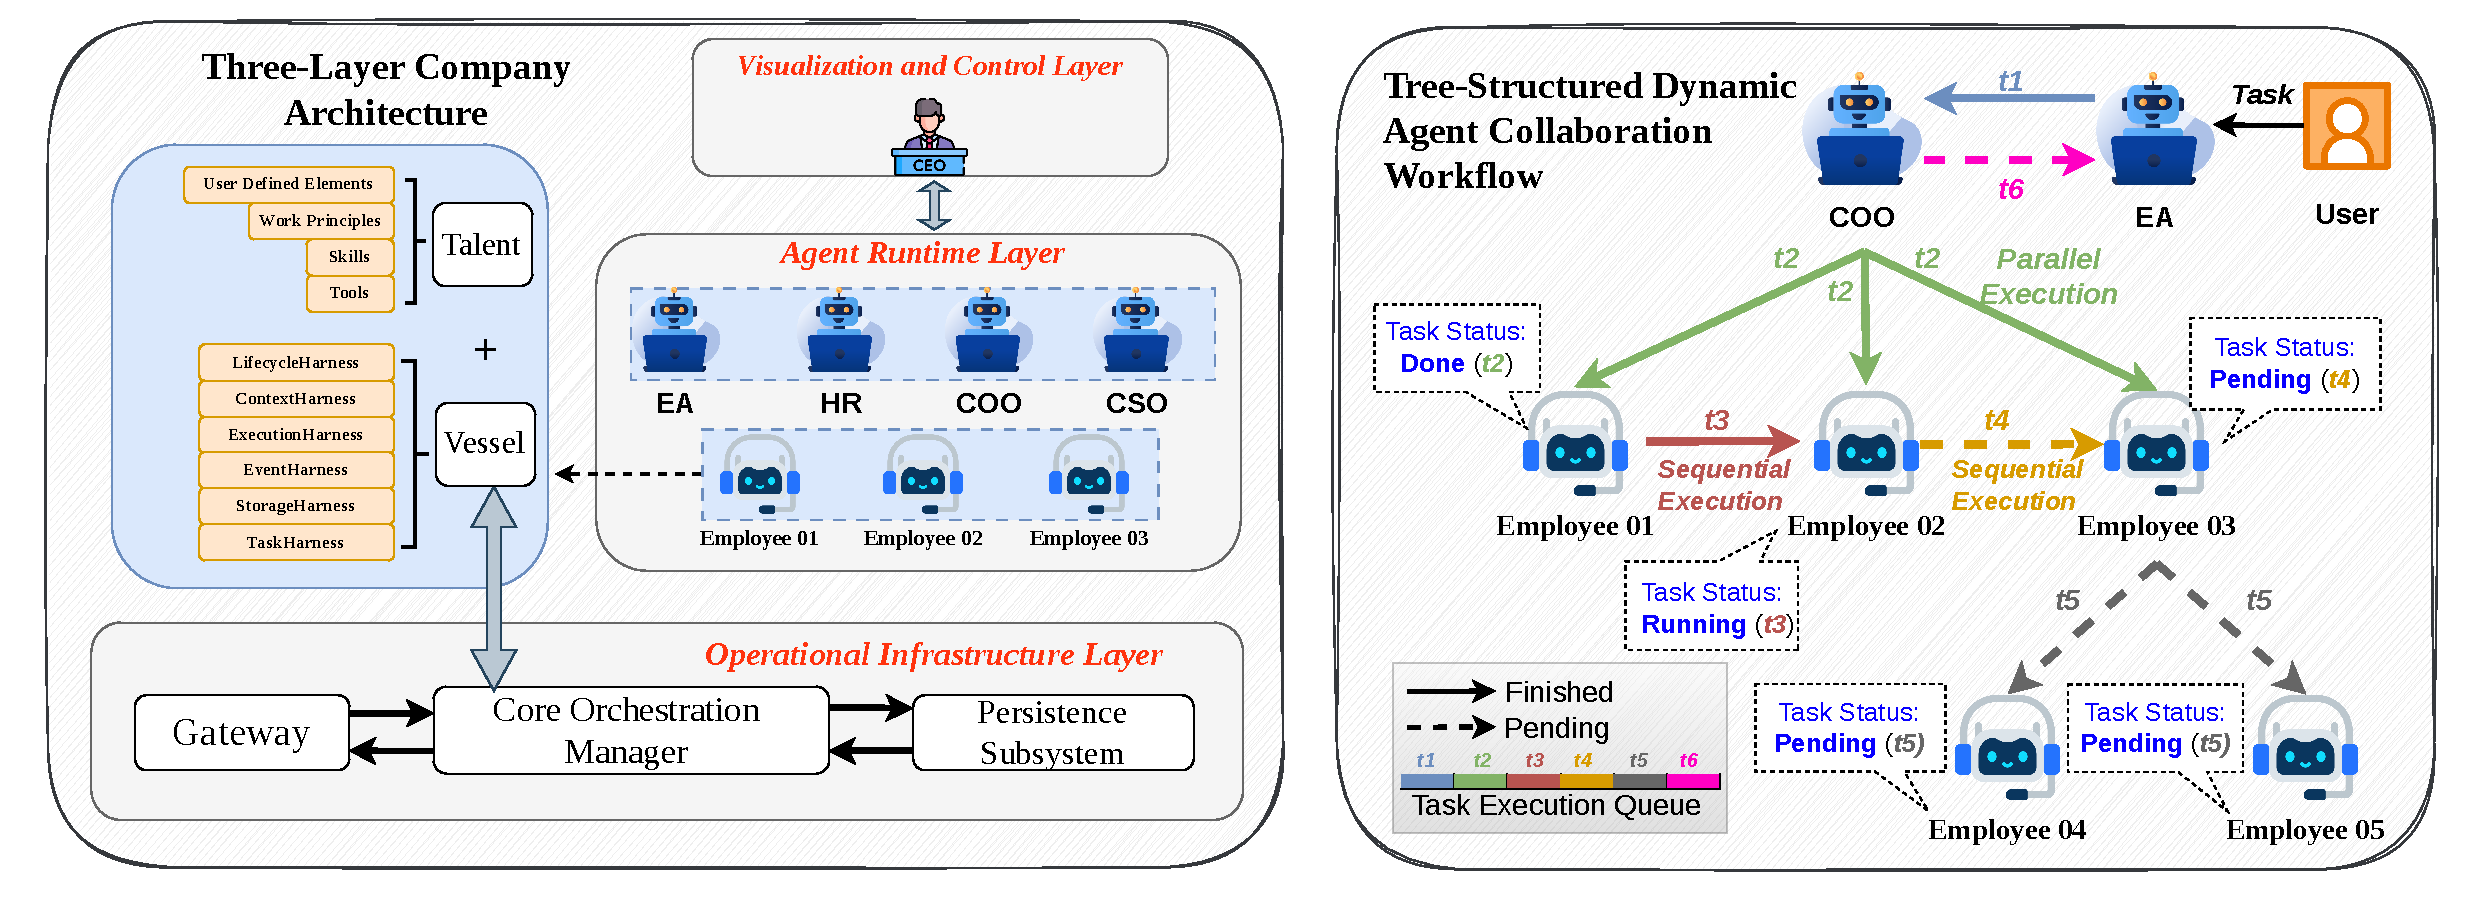
\includegraphics[width=1\textwidth]{company-structure.drawio (3).pdf}
\caption{
\textbf{Left: OMC System Architecture.} The Harness layer mediates between heterogeneous Vessels (execution backends) and the organisational platform, providing a unified contract for task dispatch, lifecycle management, and event propagation.  \textbf{Right: Dynamic Task Tree Execution.} Tasks propagate through a hierarchical AND-tree with DAG dependencies; colours represent different time steps during execution.
}
    \label{fig:arch-overview}
\end{figure}


% ─────────────────────────────────────────────────────────────────────
\subsection{Explore-Execute-Review Tree Search}
\label{sec:explore-review}
% ─────────────────────────────────────────────────────────────────────

\subsubsection{Problem: Strategy Search in a Vast Organizational Space}

Consider a company that receives a project request. The space of possible responses is enormous: the project can be decomposed in multiple ways, each subtask can be assigned to different employees, each intermediate result can be accepted, rejected, or iterated upon, and the entire decomposition can be revised after observing partial outcomes. Existing multi-agent frameworks typically handle this by either hardcoding a fixed workflow graph or allowing agents to freely negotiate, neither of which scales: fixed workflows cannot adapt to novel projects, while unconstrained negotiation provides no convergence guarantees.

% We observe that this problem shares key structural properties with game-tree search: a large branching factor, stochastic outcomes (LLM execution is non-deterministic), and the need to balance exploring new strategies against exploiting known-good ones.
We observe that this problem shares key structural properties with game-tree search: a large branching factor, stochastic outcomes from non-deterministic LLM execution, and the need to balance exploration and exploitation.
Drawing on the structural principles of Monte Carlo Tree Search (MCTS)~\cite{kocsis2006bandit}, OMC decomposes the organizational decision cycle into an \textbf{Explore-Execute-Review} loop: \emph{explore} the strategy space (select a decomposition and expand the task tree), \emph{execute} the plan (agents carry out assigned work), and \emph{review} the results (propagate quality signals to refine future decisions).

\subsubsection{Tree Structure: Nodes and Edges}

The Explore-Execute-Review loop operates over a \emph{search tree} $\mathcal{T} = (V, E_{\text{tree}}, E_{\text{dep}})$ that grows dynamically during project execution.

\paragraph{Nodes.}
Each node $v \in V$ represents an \textbf{organisational decision point}, a task at a specific granularity together with its assigned employee and current status.  Formally:
\begin{equation}
v = (d,\; e,\; \phi,\; r,\; c)
\end{equation}
where $d$ is the task description (a natural-language specification of what needs to be done), $e \in \mathcal{W} \cup \{\varnothing\}$ is the assigned employee (or $\varnothing$ if unassigned), $\phi \in \Sigma$ is the current status from the finite state machine defined in Section~\ref{sec:dag}, $r$ is the result produced upon completion (initially $\varnothing$), and $c \in \mathbb{R}_{\geq 0}$ is the accumulated execution cost.  The root node is the original project request; interior nodes are decomposition decisions; leaf nodes are atomic tasks that employees execute directly.

\paragraph{Edges.}
Two types of edges structure the tree:
\begin{itemize}[nosep]
    \item \textbf{Decomposition edges} $E_{\text{tree}} \subseteq V \times V$: a directed edge $(p, v’)$ means ``parent $p$ was decomposed into child $v’$’’.  These form a strict tree (each child has exactly one parent) and encode the \emph{strategy} chosen at the Explore stage; different decomposition choices produce different subtrees.
    \item \textbf{Dependency edges} $E_{\text{dep}} \subseteq V \times V$: a directed edge $(u, v)$ means ``$v$ cannot begin execution until $u$ is accepted’’.  These encode execution ordering constraints \emph{within} a decomposition strategy and may cross sibling branches (e.g., the frontend task depends on the API task, even though both are children of the same parent).
\end{itemize}
The combined graph $G = (V, E_{\text{tree}} \cup E_{\text{dep}})$ must be a DAG, enforced at insertion time via DFS cycle detection.

\paragraph{State Space.}
An organisational state $s \in \mathcal{S}$ is a snapshot of the full system:
\begin{equation}
s = (\mathcal{T}, \mathcal{W}, \mathcal{R})
\end{equation}
where $\mathcal{T}$ is the current search tree (node statuses, partial results), $\mathcal{W}$ is the workforce state (employee skills, workload, performance history), and $\mathcal{R}$ is the resource state (token budget, cost accumulation, time constraints).

\paragraph{Actions.}
At each decision point, the system selects from five action types that modify the tree:
\begin{equation}
\mathcal{A} = \mathcal{A}_{\text{decompose}} \cup \mathcal{A}_{\text{assign}} \cup \mathcal{A}_{\text{recruit}} \cup \mathcal{A}_{\text{review}} \cup \mathcal{A}_{\text{iterate}}
\end{equation}
$\mathcal{A}_{\text{decompose}}$ adds decomposition edges (new children under a node); $\mathcal{A}_{\text{assign}}$ binds an employee to a leaf node; $\mathcal{A}_{\text{recruit}}$ hires a new employee from the Talent Market when required capabilities are missing (Section~\ref{sec:talent-market}); $\mathcal{A}_{\text{review}}$ transitions a node’s status (accept or reject); and $\mathcal{A}_{\text{iterate}}$ creates a new root-level iteration with an updated strategy.

\paragraph{Strategies and policy.}
A \emph{strategy} $\sigma$ is a sequence of actions applied to the current state:
\begin{equation}
\sigma = (a_1, a_2, \ldots, a_m), \quad a_i \in \mathcal{A}, \quad s_{i+1} = a_i(s_i)
\end{equation}
In the Explore stage, the system must select a strategy for the current decision point.  We define a \emph{policy} $\pi$ that maps a state to a strategy:
\begin{equation}
\pi(s) \to \sigma = \bigl(\alpha_{\text{d}}(v, \{v'_1, \ldots, v'_n\}),\; \alpha_{\text{a}}(v'_1, e_1),\; \ldots,\; \alpha_{\text{a}}(v'_n, e_n)\bigr)
\end{equation}
where $v$ is the node to be expanded, $\{v'_1, \ldots, v'_n\}$ are the new child tasks, $\alpha_{\text{d}}$ denotes a decompose action, $\alpha_{\text{a}}$ denotes an assign action, and $e_i$ is the employee assigned to $v'_i$ (possibly via a recruit action if no suitable employee exists).  The composite operation $\Delta(v, e, d, D)$ applies one decompose--assign pair, creating a child node with description $d$, assigning employee $e$, and registering dependency edges $D$:
\begin{equation}
\mathcal{T}_{k+1} = \mathcal{T}_k \cup \{v_{\text{new}}\}, \quad v_{\text{new}} = \Delta(v, e, d, D)
\end{equation}
In the current implementation, $\pi$ is realised by the LLM reasoning over the project state, employee profiles, and accumulated performance history.  The LLM serves as a heuristic policy that jointly decides decomposition granularity and employee assignment.

\paragraph{The Three Stages of Explore-Execute-Review.}
Each iteration of the search loop applies $\pi$, executes the resulting strategy, and feeds back quality signals, in three stages:

\textit{Stage 1: Explore} (strategy selection and task tree expansion).
The executive agents apply $\pi(s)$ to select a strategy: how to decompose the current task and whom to assign.  This stage faces the classic exploration--exploitation trade-off: assign tasks to employees with proven track records (exploitation) or try less-tested employees, or hire a new one, to discover hidden capability (exploration).  The branching factor is unbounded, since the LLM decides decomposition granularity at runtime.

\textit{Stage 2: Execute} (agents carry out assigned work).
Each assigned employee executes its task through the Harness (Section~\ref{sec:harness}).  Each execution yields:
\begin{equation}
\mathcal{E}(v) = f_{v.e}(v.d) \to (r, c)
\end{equation}
where $r$ is the result and $c$ is the execution cost.  The internal function $f$ is determined by the agent's own loop (e.g., reasoning, tool use, code generation) and is opaque to the organisational layer.  The quality signal $q$ is produced separately in Stage~3 when a reviewer evaluates $r$.  The DAG execution layer (Section~\ref{sec:dag}) formalises the dependency resolution and termination guarantees for this stage.

\textit{Stage 3: Review} (quality signals propagate and drive iteration).
For each completed node, a reviewer (typically the node's parent owner or the COO) evaluates the result $r$ and produces a quality signal $q(v) \in \{\textsc{accept}, \textsc{reject}\}$, which triggers the corresponding status transition in the FSM.  These review decisions propagate bottom-up from leaf nodes to the root, accumulating into a signal vector per node:
\begin{equation}
\mathbf{s}(v) = \bigl(q(v),\; c(v),\; \text{status}(v)\bigr), \quad \forall v \in \text{path}(\text{leaf}, \text{root})
\end{equation}

Signals propagate until the root is reached.  Whether a node counts as resolved is defined by the AND-semantics in Section~\ref{sec:dag}.  Accumulated signals are persisted in task histories and employee progress logs, enriching the organisational context for future iterations.  Rejected results trigger re-exploration: the system returns to Stage~1 with updated context, closing the loop.

\subsubsection{Iterated Search with External Oracle}

Each project iteration ($\texttt{iter\_001}, \texttt{iter\_002}, \ldots$) corresponds to one search episode.  We define the policy update function $\Pi$ that refines the organisational policy after each iteration by incorporating execution outcomes:
\begin{equation}
\pi_{k+1} = \Pi(s_k, \pi_k, \mathcal{H}_k)
\end{equation}
where $\mathcal{H}_k = \{(v, r, c, q)\}_{v \in \text{completed}}$ is the accumulated execution history (results, costs, and review signals from all completed nodes up to iteration $k$).

The CEO (or an external customer of the company) acts as an \emph{external oracle} who provides three types of intervention: (1) \textbf{policy override}, directly rejecting or redirecting a decomposition strategy; (2) \textbf{requirement injection}, adding new constraints mid-search (``add SEO support’’, ``change the architecture’’); and (3) \textbf{iteration triggering}, deciding when to launch a new search episode and when to stop. We model this human stakeholder as a meta-level controller~\cite{russell1991right} who applies domain-informed optimal stopping, iterating when the expected improvement justifies the cost and stopping when marginal returns diminish.

This human-in-the-loop design has a practical advantage: the stakeholder prunes unpromising branches early, injects external information unavailable to the system (market signals, strategic priorities), and concentrates computation on high-value regions of the search space. The trade-off is that convergence depends on the quality of human judgment rather than on formal guarantees.

\subsubsection{Bounded Rationality and Circuit Breakers}

Real organizations cannot run infinite simulations. OMC implements bounded rationality through three mechanisms:
\begin{enumerate}
    \item \textbf{Review round limit} ($k_{\text{rev}} = 3$): $n_{\text{rev}}(v) \geq k_{\text{rev}} \implies \text{esc}(v)$
    \item \textbf{Task timeout} ($T = 3600\text{s}$): $t_{\text{exec}}(v) > T \implies \text{status}(v) \leftarrow \textsc{failed}$
    \item \textbf{Cost budget}: $\sum_{v \in \mathcal{T}} c(v) > B \implies \text{pause}$
\end{enumerate}
These mechanisms serve as a computational budget analogous to the simulation limit in tree search. Together, they guarantee that every search episode terminates in bounded time and cost under the assumption that the underlying executor (LLM, tool calls, external services) respects the timeout contract. Section~\ref{sec:dag} formalizes the stronger execution guarantees that hold within these bounds.


% ─────────────────────────────────────────────────────────────────────
\subsection{DAG-based Task Decomposition and Execution}
\label{sec:dag}
% ─────────────────────────────────────────────────────────────────────

The Explore-Execute-Review tree search and DAG execution form two complementary layers: each search \emph{iteration} corresponds to one complete DAG execution cycle, and the DAG layer returns the signals (quality, cost, time) that drive the review phase:
\begin{equation}
\mathcal{I}(s, a) = \mathcal{E}_{\text{DAG}}(\tau(s, a)) \to (r, c, q)
\end{equation}
where $\tau(s, a)$ is the task tree instance produced by decomposition action $a$ in state $s$, $\mathcal{E}_{\text{DAG}}$ is the DAG scheduler that executes all ready nodes, resolves dependencies, and propagates review signals (defined by the scheduling, propagation, and guarantee rules below), and $(r, c, q)$ are the result, cost, and quality signals returned to the EER review phase.

\subsubsection{Problem: Guaranteeing Task Completion in Dynamic Decomposition}

Once the exploration phase selects a decomposition strategy, the resulting task graph must be executed reliably. The challenge is non-trivial: tasks may depend on each other in arbitrary DAG patterns, employees may fail or produce unacceptable results, and the system must recover from crashes without losing progress. Without formal guarantees, a multi-agent system risks silent stalls: tasks that never reach a terminal state, dependencies that permanently block downstream work, or review loops that cycle indefinitely.

We formalize task execution as scheduling over an AND-tree augmented with dependency edges, where a finite state machine governs each node’s lifecycle with termination guarantees under bounded retry and finite resource constraints.

\subsubsection{AND-Tree with DAG Dependencies}

The task tree $\mathcal{T} = (V, E_{\text{tree}}, E_{\text{dep}})$ and its DAG invariant were defined in Section~\ref{sec:explore-review}.  Here we specify the execution semantics that govern how this tree is scheduled and completed.

\paragraph{AND-Semantics.}
A node $v$ is \emph{resolved} according to the following recursive definition:
\begin{equation}
\text{resolved}(v) \iff \begin{cases} v.\phi \in \{\textsc{accepted}, \textsc{finished}\} & \text{if } v \text{ is a leaf} \\ \forall v' \in \text{children}(v) \setminus S : \text{resolved}(v') & \text{otherwise} \end{cases}
\end{equation}
where $S$ is the set of system node types (review requests, watchdog nudges).  This AND-semantics is the key structural guarantee: completion \emph{must} propagate bottom-up from leaves through the entire tree.  No subtask can be silently dropped.

\subsubsection{Task Lifecycle State Machine}

Each task node follows a finite state machine $M = (\Sigma, \delta, s_0, F)$ where:
\begin{itemize}
    \item $\Sigma = \{\textsc{pending}, \textsc{processing}, \textsc{holding}, \textsc{completed}, \textsc{accepted}, \textsc{failed}, \textsc{blocked}, \textsc{finished}, \textsc{cancelled}\}$
    \item $s_0 = \textsc{pending}$, \quad $F = \{\textsc{finished}, \textsc{cancelled}\}$ (terminal states)
\end{itemize}

The transition function $\delta$ is shown in Figure~\ref{fig:task-states}.

\begin{figure}[H]
    \centering
    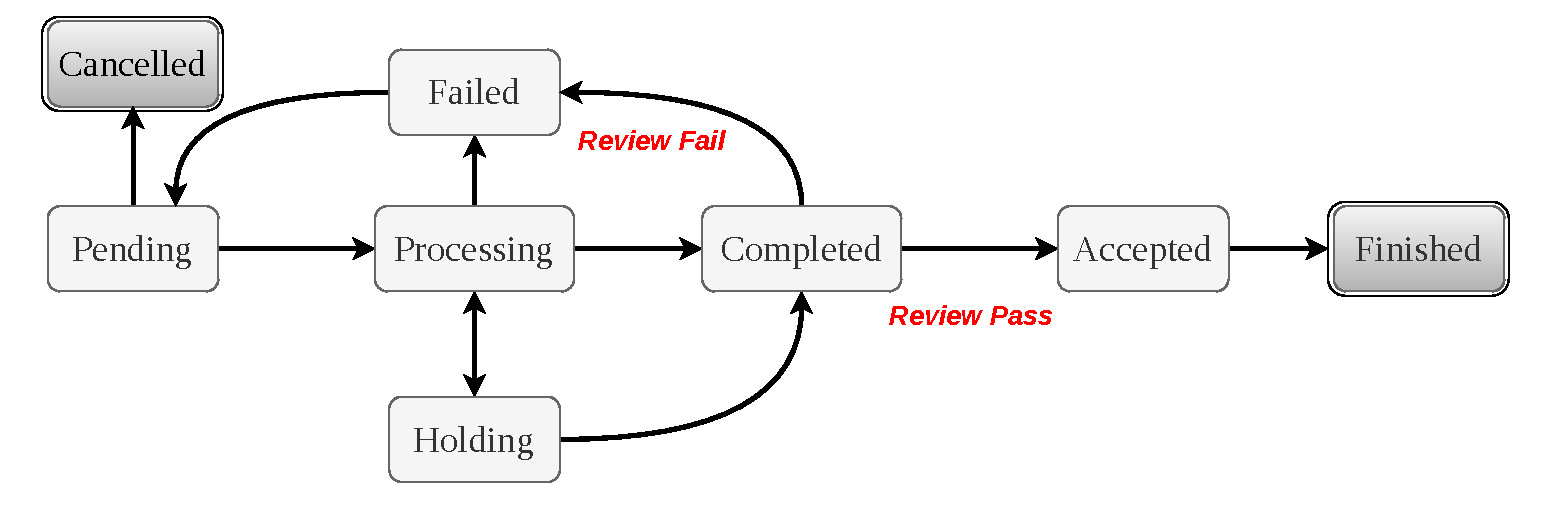
\includegraphics[width=0.9\textwidth]{taskflow.drawio.pdf}
\caption{\textbf{Task state machine.} Double-bordered states are terminal. The \textsc{completed}$\to$\textsc{accepted} transition requires explicit supervisor review, preventing unverified results from propagating downstream.}
\label{fig:task-states}
\end{figure}

Two design choices are critical (Figure~\ref{fig:task-states}). First, \textsc{completed}$\to$\textsc{accepted} requires explicit supervisor review, which prevents hallucinated or incorrect results from unblocking dependent tasks. Second, the \textsc{failed}$\to$\textsc{processing} retry path is bounded by a maximum retry count $k_{\text{retry}}$; exceeding this limit triggers escalation, guaranteeing that no node cycles indefinitely.

\subsubsection{Scheduling and Dependency Resolution}

A node $v$ becomes executable when its dependency constraints are satisfied:
\begin{equation}
\text{ready}(v) \iff \text{status}(v) = \textsc{pending} \;\wedge\; \forall u \in \text{deps}(v) : \text{status}(u) \in \{\textsc{accepted}, \textsc{finished}\}
\end{equation}

The scheduler selects the first ready node per employee in FIFO order, subject to a mutual exclusion invariant: $|\text{running}(e)| \leq 1$ for all employees $e$. When a node reaches a resolved state, dependency resolution propagates forward through the DAG:
\begin{itemize}
    \item Dependent nodes with all dependencies resolved are scheduled for execution.
    \item Dependent nodes with failed dependencies are marked \textsc{blocked} (or cascade-cancelled if the failure is non-recoverable).
    \item Cascade cancellation implements transitive closure: $\text{cancel}(v) \implies \forall w : v \in \text{deps}(w) \implies \text{cancel}(w)$.
\end{itemize}

\subsubsection{Bottom-Up Completion Propagation}

When a leaf node completes and passes review, the AND-semantics trigger recursive propagation: if all children of a parent are resolved, the parent auto-promotes to \textsc{completed}$\to$\textsc{accepted}$\to$\textsc{finished}, which in turn triggers its own parent’s resolution check, and so on up to the project root. This bottom-up propagation ensures that project completion is a \emph{derived} property of subtask completion, not a separately maintained flag.

A deadlock detector provides a safety net: if all non-root nodes are in terminal or blocked states but the root has not resolved, the project is marked as failed, preventing silent stalls.

\subsubsection{Formal Guarantees}

The combined design provides seven invariants:

\begin{enumerate}
    \item \textbf{DAG Invariant}: $G = (V, E_{\text{tree}} \cup E_{\text{dep}})$ is always acyclic (enforced at insertion).
    \item \textbf{Mutual Exclusion}: $|\text{running}(e)| \leq 1$ for all employees $e$, i.e., each employee executes at most one task at a time.
    \item \textbf{Schedule Idempotency}: repeated scheduling of the same node is a no-op, ensuring that crash recovery or concurrent events never cause duplicate task execution.
    \item \textbf{Review Termination}: at most $k_{\text{rev}}$ reviews per parent before escalation to a higher-level supervisor.
    \item \textbf{Cascade Completeness}: cancellation propagates to all transitive dependents.
    \item \textbf{Dependency Completeness}: every resolved-state transition triggers forward dependency resolution; no dependent is left permanently \textsc{pending}.
    \item \textbf{Recovery Correctness}: after crash, \textsc{processing} nodes reset to \textsc{pending} (re-executed), and all \textsc{pending} nodes with resolved dependencies are re-scheduled, ensuring the system resumes from a consistent state.
\end{enumerate}


% ─────────────────────────────────────────────────────────────────────
\subsection{Talent Market: Where Agents Come From}
\label{sec:talent-market}
% ─────────────────────────────────────────────────────────────────────

OMC integrates a community-driven Talent Market\,\footnote{\url{https://one-man-company.com/}} as a native capability layer.  Rather than synthesising agents from descriptive prompts, a practice prone to capability hallucination. Instead, OMC recruits from a pool of community-verified, benchmark-validated implementations and provisions them through an automated hiring pipeline.

\subsubsection{What the Talent Market Provides}

Each Talent on the marketplace is a complete, ready-to-deploy agent package: system prompts and role definitions, tool configurations and MCP integrations, skill scripts, domain knowledge files, and benchmark results that document the agent's verified capabilities.  Talents span a wide range of specialisations (software engineers, data analysts, content writers, art designers, QA testers, research analysts, among others), each grounded in executable artefacts rather than descriptive claims.  Because Talents are decoupled from Vessels (Section~\ref{sec:harness}), the same Talent can be deployed on any supported runtime (LangGraph, Claude CLI, script-based), and the same OMC instance can recruit Talents built on entirely different agent families to form a heterogeneous team.

The marketplace supports three sourcing channels: (1)~\textbf{community-contributed Talents}, open-source agent packages uploaded and peer-reviewed by the community; (2)~\textbf{AI-recommended assembly}, an AI-powered engine that discovers suitable skills and tools from the web and assembles them into functional Talent packages, mitigating the cold-start problem for underserved domains; and (3)~\textbf{internal promotion}, high-performing employees whose refined profiles and accumulated skills are packaged and shared back to the marketplace.

\subsubsection{Hiring Pipeline}

When the policy $\pi(s)$ requires a capability absent from the current workforce, triggering a recruit action $\alpha_{\text{r}} \in \mathcal{A}_{\text{recruit}}$, the HR agent queries the Talent Market, compiles a ranked shortlist based on skill match and community ratings, and presents candidates to the CEO for approval.  Upon selection, the automated pipeline provisions the Talent with a Vessel, assigns a desk, configures tool access, and registers the new employee in the organisational hierarchy, all without manual setup.  This on-demand recruitment closes the loop between capability demand (what the project needs) and supply (what the community has built), enabling OMC to tackle projects across arbitrary domains without pre-configuring a fixed team.


% ─────────────────────────────────────────────────────────────────────
\subsection{Self-Evolution: How Agents and the Organisation Improve}
\label{sec:self-evolution}
% ─────────────────────────────────────────────────────────────────────

The components described so far handle execution, but not learning.  In a real company, employees grow through one-on-ones with their manager, projects end with post-mortems, and periodic performance reviews create accountability.  OMC implements all three.

\subsubsection{Individual-Level Evolution}

Each agent maintains a persistent, auto-updating profile comprising a cross-task progress log and LLM-summarised working principles.  Two triggers drive individual reflection:

\begin{enumerate}[nosep]
    \item \textbf{CEO one-on-one.}  After each one-on-one session with the CEO, the agent performs structured self-reflection: reviewing the CEO's feedback, identifying gaps between expected and actual behaviour, and updating its working principles accordingly.  This mirrors the manager--report one-on-one in human organisations, where direct feedback drives targeted skill development.
    \item \textbf{Post-task review.}  Upon task completion, the agent reviews its own execution trace (decisions made, tools invoked, obstacles encountered) and appends a summary to its progress log.  Over successive tasks, this log accumulates a trajectory of lessons learned that enriches the agent's context for future work.
\end{enumerate}

Critically, these updates modify the agent's Talent artefacts (working principles, guidance notes) rather than the underlying foundation model, enabling continuous improvement without retraining.  In the formal model, updated working principles are reflected in the workforce state $\mathcal{W}$, so subsequent calls to $\pi(s)$ see the improved agent profiles.

\subsubsection{Organisation-Level Evolution}

At the project level, OMC conducts structured retrospectives that mirror real-world project post-mortems.  When a project reaches completion, the COO convenes a retrospective session:

\begin{enumerate}[nosep]
    \item Each participating employee submits a self-assessment summarising key decisions, obstacles encountered, and solutions adopted.
    \item The COO aggregates these self-assessments with objective signals: per-task retry counts, review rejection reasons, and resource consumption.
    \item The retrospective distils findings into two outputs: (a)~\emph{individual feedback} that updates each employee's working principles, and (b)~\emph{organisational SOPs} that codify effective patterns for future projects (e.g., ``mandate API contract review before frontend--backend integration'').
\end{enumerate}

These SOPs are persisted as workflow documents and automatically injected into relevant agents' contexts in subsequent projects, ensuring that organisational knowledge accumulates across projects rather than remaining confined to individual agent memories.

\subsubsection{Performance Review and HR Lifecycle}

To create accountability and prevent capability stagnation, OMC implements a formal performance review pipeline inspired by real-world HR practices:

\begin{itemize}[nosep]
    \item \textbf{Periodic review trigger.}  Every three projects, the HR agent automatically initiates a performance evaluation for each participating employee, assessing task completion quality, review pass rates, and collaboration effectiveness.
    \item \textbf{Performance Improvement Plan (PIP).}  An employee who fails three consecutive performance reviews enters a formal PIP, receiving targeted coaching, adjusted task assignments, and closer supervision.
    \item \textbf{Automated offboarding.}  If an employee under PIP fails one additional review, the system triggers automatic dismissal: the agent's Vessel is deprovisioned, its desk is freed, and the capability gap is flagged for re-recruitment from the Talent Market.
\end{itemize}

This lifecycle management closes the loop between the Talent Market (Section~\ref{sec:talent-market}) and organisational evolution: underperforming agents are replaced by fresh recruits, while high-performing agents accumulate experience that makes them increasingly effective.  We are not aware of prior work that applies structured HR protocols (performance reviews, PIP, formal offboarding) to AI agent lifecycle management.


% =====================================================================
\section{Comparative Analysis}
\label{sec:comparison}
% =====================================================================

\subsection{Architectural Taxonomy}

\begin{table}[H]
\centering
\caption{Architectural comparison across systems.  ``Agent--Platform Contract'' indicates the mechanism through which agents interact with the orchestration platform.}
\label{tab:archcomp}
\footnotesize
\renewcommand{\arraystretch}{1.2}
\setlength{\tabcolsep}{3pt}
\begin{tabularx}{\textwidth}{@{}>{\raggedright\arraybackslash}p{2.1cm}
>{\centering\arraybackslash}p{1.6cm}
>{\centering\arraybackslash}p{1.8cm}
>{\centering\arraybackslash}p{1.8cm}
>{\centering\arraybackslash}p{1.7cm}
>{\centering\arraybackslash}p{1.4cm}
>{\centering\arraybackslash}X
>{\centering\arraybackslash}X@{}}
\toprule
\textbf{System} & \textbf{Abstraction} & \textbf{Execution Model} & \textbf{Agent--Platform Contract} & \textbf{State Mgmt.} & \textbf{Multi-Exec.} & \textbf{Self-Evol.} & \textbf{Org. Learn.} \\
\midrule
\textbf{OMC} & OS-inspired & On-demand & 6 typed interfaces & Disk & 3 backends & \textcolor{green}{\checkmark} & \textcolor{green}{\checkmark} \\
MetaGPT / ChatDev & Pipeline & Sequential & Implicit (SOP) & In-memory & \textcolor{red}{$\times$} & \textcolor{red}{$\times$} & \textcolor{red}{$\times$} \\
AutoGen / LangGraph & Library & Event / Graph & Callbacks & Checkpoints & \textcolor{red}{$\times$} & \textcolor{red}{$\times$} & \textcolor{red}{$\times$} \\
CrewAI / Agno & Framework & Seq. / parallel & Class inherit. & App-defined & \textcolor{red}{$\times$} & \textcolor{red}{$\times$} & \textcolor{red}{$\times$} \\
OpenHands & Platform & Agent loop & Built-in runtime & Sandboxed & \textcolor{red}{$\times$} & \textcolor{red}{$\times$} & \textcolor{red}{$\times$} \\
AIOS & OS kernel & Scheduled & OS syscalls & OS-managed & \textcolor{red}{$\times$} & \textcolor{red}{$\times$} & \textcolor{red}{$\times$} \\
AgentScope & Platform & Distributed & Partial & App-defined & \textcolor{red}{$\times$} & \textcolor{red}{$\times$} & \textcolor{red}{$\times$} \\
\bottomrule
\end{tabularx}
\end{table}

Table~\ref{tab:archcomp} reveals three structural gaps that OMC addresses.

\paragraph{Agent--platform contract.}
Most frameworks couple agents to the platform through implicit mechanisms: MetaGPT and ChatDev encode coordination in fixed SOPs, AutoGen and LangGraph rely on framework-specific callbacks, and CrewAI uses class inheritance.  These approaches tightly bind agent identity to a single execution model, making it difficult to swap backends or integrate agents from different families.  OMC's six typed Harness interfaces (Section~\ref{sec:harness}) provide a formal, substitutable contract that decouples agent identity from execution substrate, enabling three heterogeneous backends to coexist within a single orchestration loop.  AIOS also positions itself as an OS kernel, but its syscall interface targets resource scheduling rather than agent identity separation.

\paragraph{Multi-backend execution.}
OMC is the only system in the comparison that supports multiple execution backends simultaneously.  This is a direct consequence of the Talent--Vessel separation: because the orchestration layer interacts exclusively with the Harness contract, it is agnostic to whether a task is executed by a LangGraph agent, a Claude CLI session, or a script-based process.  Other systems either restrict execution to a single runtime (OpenHands, AIOS) or delegate backend choice entirely to the application developer (AutoGen, AgentScope).

\paragraph{Self-evolution and organisational learning.}
No other system in the comparison implements both individual self-evolution and organisational learning.  Existing frameworks treat agents as stateless executors that are re-instantiated for each task; any adaptation must be implemented externally by the user.  OMC's self-evolution mechanisms (Section~\ref{sec:self-evolution}), including post-task reflection, project retrospectives, and the HR performance review pipeline, enable persistent improvement at both the agent and organisation levels without requiring model retraining.


% =====================================================================
\section{Experiments}
\label{sec:experiments}
% =====================================================================

We evaluate OMC on PRDBench, a recently proposed benchmark for assessing LLM-based code agents in realistic software development scenarios.  PRDBench consists of 50 project-level tasks spanning over 20 domains, where each task is defined by a structured Product Requirement Document (PRD) along with comprehensive evaluation criteria.  Each test case provides high-level requirements, auxiliary data, detailed test plans, and executable evaluation scripts, enabling end-to-end assessment of an agent’s ability to interpret requirements, decompose tasks, implement solutions, and satisfy functional constraints.  Unlike traditional benchmarks that focus on isolated code generation or unit-level correctness, PRDBench evaluates agents at the project level, requiring long-horizon reasoning, hierarchical task decomposition, and coordinated multi-agent execution, making it particularly suitable for evaluating OMC.

\subsection{Experimental Setup}

For the agent setup, in addition to our founding agent (a LangGraph-based agent using the Gemini 2.1 Flash Lite Preview model), the HR recruited three specialized employees from the Talent Market at the outset of the first PRD project. The first is a Software Engineer (a Claude Code-based agent with the superpowers plugin \footnote{\url{https://github.com/obra/superpowers}}), the second is a Software Architect (a Claude Code-based agent from the agency-agents project \footnote{\url{https://github.com/msitarzewski/agency-agents}}), and the third is a Code Reviewer, also sourced from the agency-agents project.

We follow the official DEV mode setting, in which each system receives the PRD as a one-shot input and must complete the task without iterative feedback or external intervention, with final outputs directly evaluated by automated scripts. We compare OMC against the baseline results reported in PRDBench under the same setting, using \textbf{Success Rate} as the primary metric, defined as the percentage of tasks successfully completed. In addition, we report the \textbf{cost overhead} of each method (e.g., token usage or API cost) to reflect the efficiency of different agent systems under the same zero-shot conditions.

\subsection{Main Results}

% \begin{table}[H]
\begin{table}[t]
\centering
\caption{Performance comparison on PRDBench.}
\label{tab:prdb_results}
\small
\begin{tabular}{lcccc}
\toprule
\textbf{AgentType} & \textbf{Method} & \textbf{Success Rate (\%)} & \textbf{Cost (\$)} \\
\midrule
Minimal & GPT-5.2 & 62.49 & - \\
Minimal & Claude-4.5 & 69.19 & - \\
Minimal & Gemini-3-Pro & 22.76 & - \\
Minimal & Qwen3-Coder & 43.84 & - \\
Minimal & Kimi-K2 & 20.52 & - \\
Minimal & DeepSeek-V3.2 & 40.11 & - \\
Minimal & GLM-4.7 & 38.39 & - \\
Minimal & Minimax-M2 & 17.60 & - \\
Commercial & CodeX & 62.09 & - \\
Commercial & Claude Code & 56.65 & - \\
Commercial & Gemini CLI & 11.29 & - \\
Commercial & Qwen Code & 39.91 & - \\ \hline
\textbf{Multi-agent} & \textbf{\makecell{Ours (Claude Code Sonnet 4.6 \\+ Gemini 3.1 Flash Lite Preview)}} & \textbf{84.67 (+15.48)} & \textbf{345.59} \\
\bottomrule
\end{tabular}
\end{table}

As shown in Table~\ref{tab:prdb_results}, OMC achieves the highest success rate (84.67\%) across all systems, surpassing all baselines.  The total cost of \$345.59 across 50 tasks (approximately \$6.91 per task) reflects the overhead of multi-agent coordination; cost data for baselines was not reported in PRDBench, so a direct cost-efficiency comparison is not possible.

OMC's strong performance stems from its organisation-centric design.  First, the dynamic task tree enables adaptive and fine-grained task decomposition during execution, allowing the system to adjust workflows based on intermediate results rather than relying on fixed pipelines.  Second, the enforced \textsc{completed}$\to$\textsc{accepted} review mechanism acts as a built-in verification layer, effectively reducing hallucinated outputs and preventing error propagation across subtasks.  Third, the Vessel--Talent abstraction supports heterogeneous agent integration, enabling the system to recruit and coordinate specialised capabilities when needed.  Together, these mechanisms improve both execution reliability and success rate under the challenging zero-shot DEV setting.  Figure~\ref{fig:tree-task-example} shows an example of the hierarchical task decomposition produced by OMC during a PRDBench task.

\begin{figure}[H]
    \centering
    \includegraphics[width=0.9\textwidth]{ONE MAN COMPANY.pdf}
    \caption{
\textbf{Example of tree-structured task decomposition in OMC.}  The root project is iteratively decomposed into subtasks with explicit dependency edges; leaf nodes are executed by assigned employees.
}
    \label{fig:tree-task-example}
\end{figure}

\subsection{Case Study}

\subsubsection{Dynamic Team Assembly for Content Generation}
\label{sec:case-content}

We illustrate OMC's dynamic team assembly and cross-model collaboration through a
content-generation task in which the CEO instructs the system to assemble a
search-and-writing team, produce a weekly trend summary of hot AI Agent repositories
on GitHub, and email the finished article with real links to a designated address.
The entire company is triggered by a \textbf{single} CEO prompt:

\begin{mdframed}[
  linewidth=0.8pt,
  linecolor=black!40,
  backgroundcolor=black!2,
  innertopmargin=10pt,
  innerbottommargin=10pt,
  innerleftmargin=14pt,
  innerrightmargin=14pt,
  roundcorner=4pt
]
\sloppy
\noindent\texttt{Assemble a search-and-writing team, produce a weekly trend summary article of the hottest AI Agent repositories on GitHub from the past week, and email it to me upon completion with links included, all repositories must be real. Send to joedoe@email.com.}
\end{mdframed}



\noindent The only human involvement throughout the entire execution consisted of submitting the prompt above and selecting employees from the HR-compiled candidate shortlist; all subsequent planning, coordination,
execution, and delivery were performed autonomously by the system (Figure~\ref{fig:case-content}).

\begin{figure}[H]
\centering
\begin{minipage}[b]{0.30\textwidth}
    \centering
    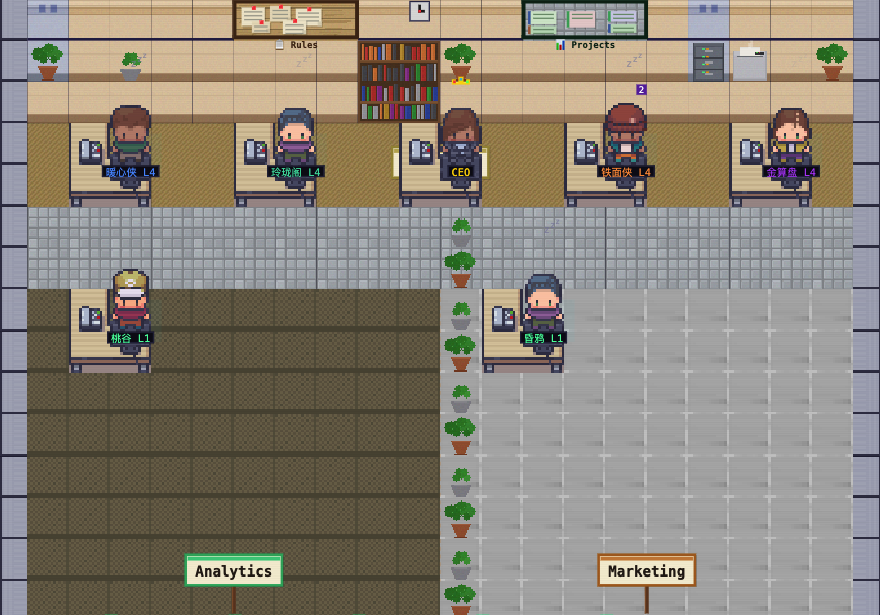
\includegraphics[width=\textwidth]{news-team.png}\\
    \vspace{2pt}
    {\small(a) Assembled team workspace}
\end{minipage}
\hfill
\begin{minipage}[b]{0.28\textwidth}
    \centering
    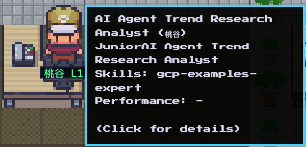
\includegraphics[width=\textwidth]{trend-researcher.png}\\
    \vspace{2pt}
    {\small(b) AI Agent Trend Research Analyst}

    \vspace{8pt}

    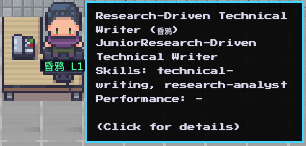
\includegraphics[width=\textwidth]{writer-2.png}\\
    \vspace{2pt}
    {\small(c) Research-Driven Technical Writer}
\end{minipage}
\hfill
\begin{minipage}[b]{0.36\textwidth}
    \centering
    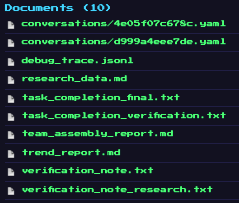
\includegraphics[width=\textwidth]{materials.png}\\
    \vspace{2pt}
    {\small(d) Project output documents}

    \vspace{8pt}

    
\includegraphics[width=\textwidth]{cost.png}\\
    \vspace{2pt}
    {\small(e) Cost \& token breakdown}
\end{minipage}

\caption{
    \textbf{Content-generation case study: team assembly, recruited agents, output artifacts, and cost breakdown.}
    (a) The OMC company workspace after team assembly, with the newly hired agents (L1) seated in the Analytics and Marketing departments.
    (b)--(c) Profile cards of the two recruited Talents: an AI Agent Trend Research Analyst and a Research-Driven Technical Writer.
    (d) Project documents produced autonomously, including \texttt{research\_data.md}, \texttt{trend\_report.md}, and verification logs.
    (e) Cost and token usage breakdown across all participating employees, totalling \$4.49.
}
\label{fig:case-content}
\end{figure}


The \textbf{EA} decomposes the directive into two sequential phases and forwards
Phase~1 to \textbf{HR}, which queries the Talent Market, compiles a ranked shortlist,
and, upon CEO approval, provisions a \textbf{Researcher} (GPT-4o) and a
\textbf{Writer} (Claude Sonnet~4) with appropriate Vessels.
Once the team is assembled, the \textbf{COO} constructs a dynamic task tree and
dispatches Phase~2: the Researcher collects verified GitHub repository links and
summaries into \texttt{research\_data.md}, and the Writer drafts a comprehensive
trend report and delivers it via email. The entire pipeline completes in under
10 minutes at a total cost of approximately \$4.48.

We manually verified all repository links and star counts reported in the
autonomously generated article, confirming that every entry is real and accurate. The final article delivered to the CEO is reproduced
in Appendix~\ref{appendix:github-report}.
\subsubsection{Game Development}


We illustrate OMC's dynamic team assembly and cross-model collaboration through a web-based street fight game development case study, serving as a concrete example of human--AI co-operation within the OMC framework. The entire company is triggered by a single CEO prompt:

\begin{mdframed}[
  linewidth=0.8pt,
  linecolor=black!40,
  backgroundcolor=black!2,
  innertopmargin=10pt,
  innerbottommargin=10pt,
  innerleftmargin=14pt,
  innerrightmargin=14pt,
  roundcorner=4pt
]
\sloppy
\noindent\texttt{Create a street-fighting web game with polished, high-quality visuals. The game should feature a playable character with smooth, fluid animations for every action and polished icon design, clean UI layouts. Ensure that each action is represented with well-crafted animation frames to create responsive and satisfying gameplay. Your colleague, the game evaluator, can be reached at: joedoe@email.com.}
\end{mdframed}

Following the hiring process, two employees have been recruited: a \textbf{Game Developer} powered by Claude Sonnet 4, and an \textbf{Art Designer} powered by Gemini 2.5 augmented with the NanoBanana tool. Upon receiving the CEO prompt, the COO constructs a dynamic task tree and dispatches specific task instructions to each employee. The Art Designer takes the first turn, generating a full set of character action images (idle, walk, kick, hurt) while the Game Developer waits. Once the Art Designer completes the visual assets, the Game Developer integrates them into the game codebase, assembling the playable prototype.

\begin{figure}[H]
\centering
\begin{minipage}[b]{0.30\textwidth}
    \centering
    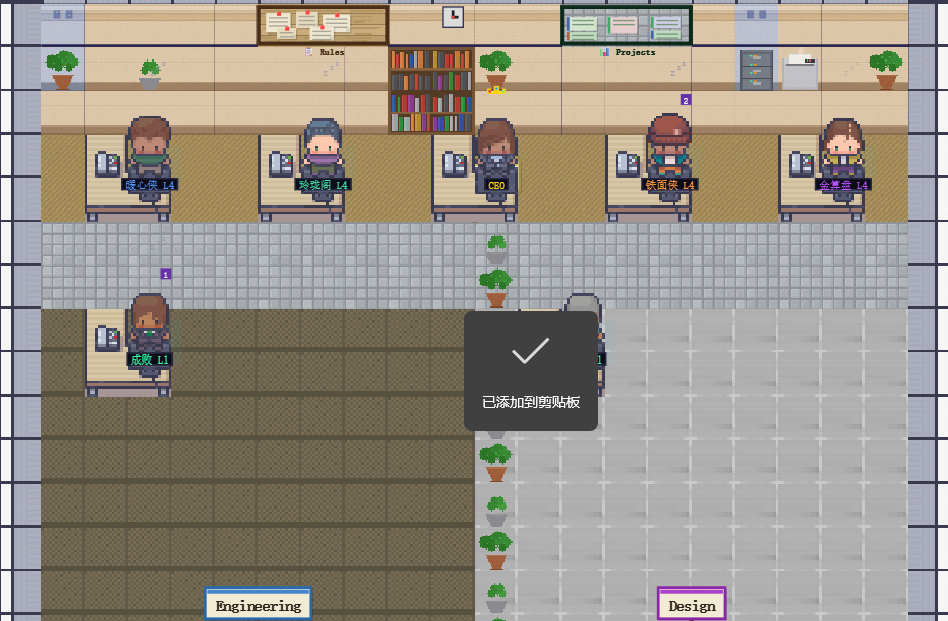
\includegraphics[width=\textwidth]{GAME-workflow/1.png}\\
    \vspace{2pt}
    {\small(a) Assembled team workspace}
    \vspace{8pt}
    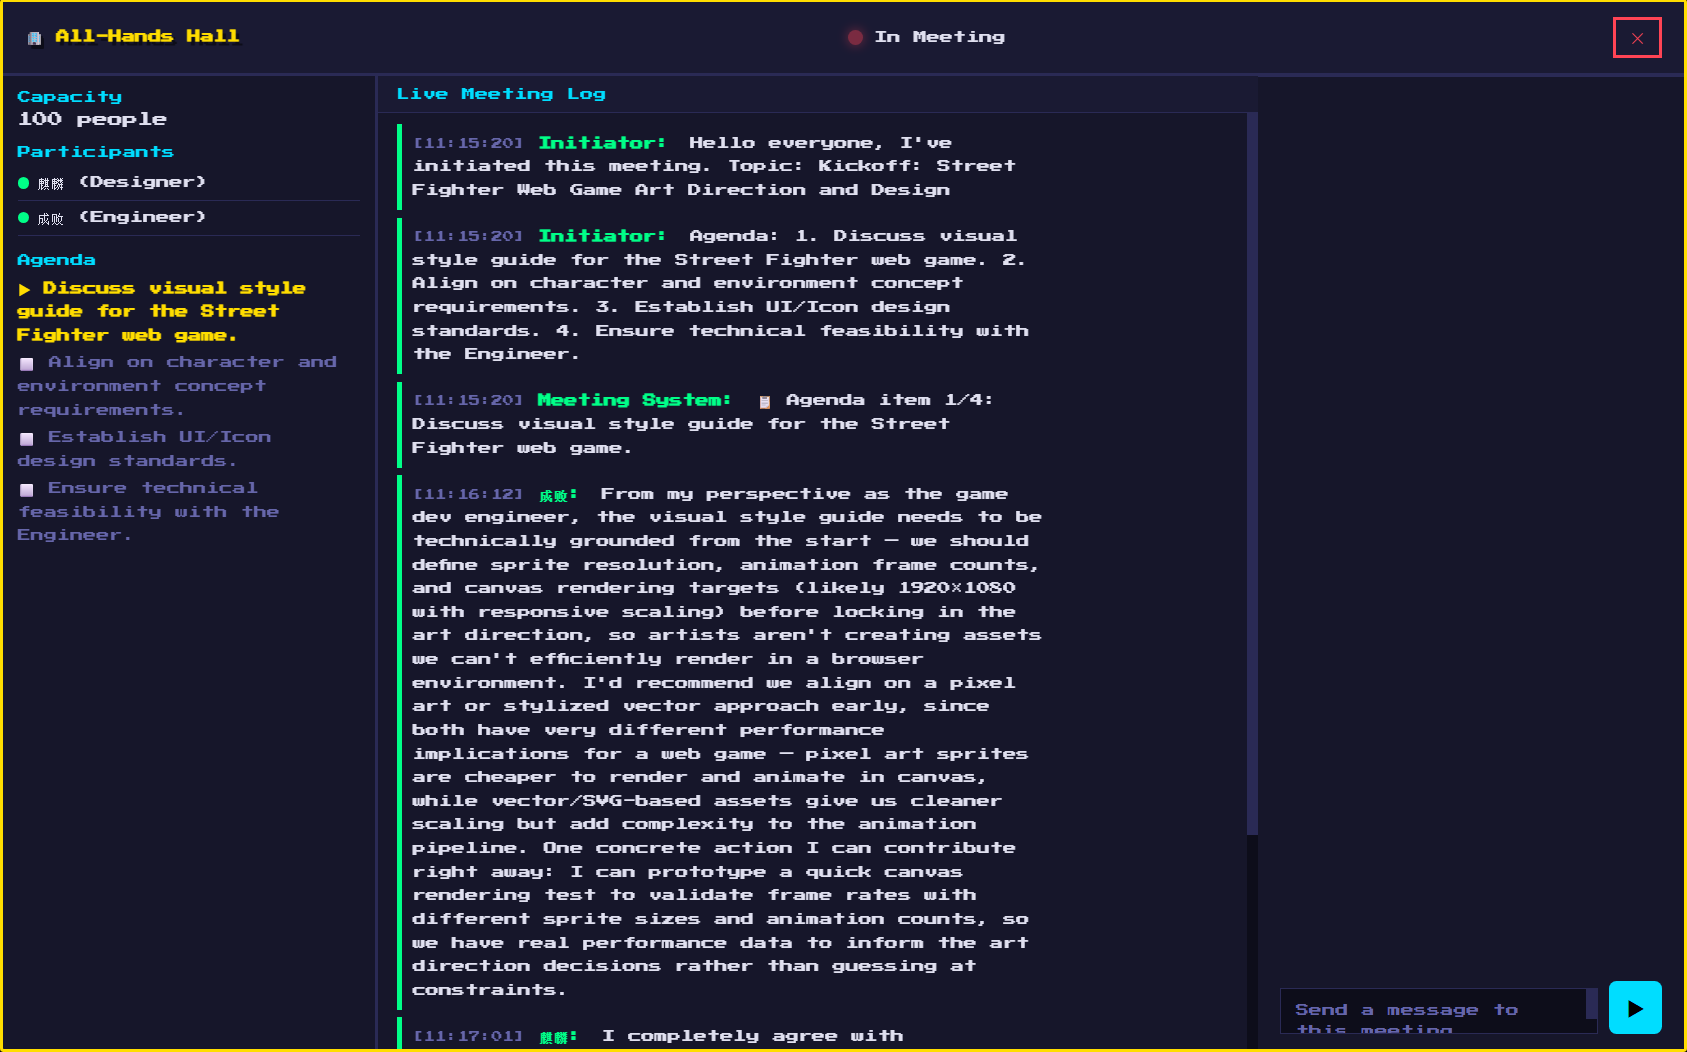
\includegraphics[width=\textwidth]{GAME-workflow/2.png}\\
    \vspace{2pt}
    {\small(b) Group meeting: Game Developer \& Art Designer}
\end{minipage}
\hfill
\begin{minipage}[b]{0.30\textwidth}
    \centering
    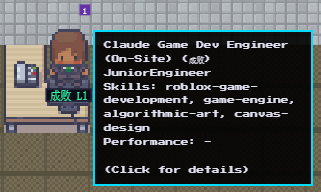
\includegraphics[width=\textwidth]{GAME-workflow/3.png}\\
    \vspace{2pt}
    {\small(c) Game Developer AI Agent}
    \vspace{8pt}
    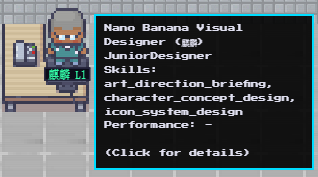
\includegraphics[width=\textwidth]{GAME-workflow/4.png}\\
    \vspace{2pt}
    {\small(d) Art Designer AI Agent}
\end{minipage}
\hfill
\begin{minipage}[b]{0.30\textwidth}
    \centering
    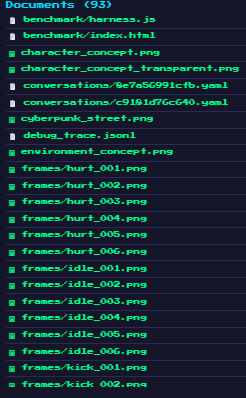
\includegraphics[width=\textwidth]{GAME-workflow/5.png}\\
    \vspace{2pt}
    {\small(e) Project output documents}
    \vspace{8pt}
    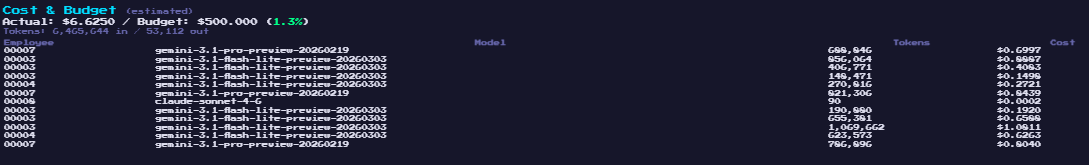
\includegraphics[width=\textwidth]{GAME-workflow/6.png}\\
    \vspace{2pt}
    {\small(f) Cost \& token breakdown}
\end{minipage}
\caption{
    \textbf{Street fight game case study: team assembly, recruited agents, output artifacts, and cost breakdown.}
    (a) The OMC company workspace after team assembly, with the newly hired agents (L1) seated in the Game Development and Art departments.
    (b) Group meeting between the Game Developer and Art Designer agents collaborating on game design.
    (c)--(d) Profile cards of the two recruited Talents: a Game Developer AI Agent and an Art Designer AI Agent.
    (e) Project documents produced autonomously, including \texttt{game\_design.md}, \texttt{asset\_list.md}, and verification logs.
    (f) Cost and token usage breakdown across all participating employees.
}
\label{fig:case-game}
\end{figure}



The initial build is then forwarded to the human evaluator at \texttt{joedoe@email.com} for quality assessment. The evaluator identifies a critical issue: the generated sprite sheets are not properly segmented, causing individual action frames to render incorrectly in-game. This feedback is relayed back through the EA and COO, who deliberate on a remediation strategy. Rather than patching the issue ad hoc, they decide to extend the system's capabilities by creating a \textbf{new skill} that equips the Art Designer with the ability to programmatically slice composite sprite sheets into individual, correctly-indexed sub-images. Armed with this new skill, the Art Designer successfully reprocesses all action assets, producing clean, well-separated animation frames. The Game Developer then re-integrates the corrected assets, and the final product is delivered to the evaluator. The complete workflow is illustrated in Figure~\ref{fig:case-game}, and the corresponding task tree with iterative feedback is shown in Figure~\ref{fig:game-task-tree}.

\begin{figure}[H]
    \centering
    \includegraphics[width=0.9\textwidth]{gamedemo.drawio.png}
    \caption{
\textbf{Game development task tree: iterative decomposition with human-in-the-loop feedback.}  The evaluator's rejection triggers re-exploration, creating a new skill for the Art Designer and re-executing the asset pipeline.
}
    \label{fig:game-task-tree}
\end{figure}








% \subsubsection{Software Development}
% \label{sec:case-software}

% We demonstrate OMC's end-to-end software development workflow using a representative scenario in which the CEO requests a Kanban-style project management web application. The \textbf{EA} receives the project brief, decomposes it into a structured task specification covering functional modules (authentication, board management, frontend UI, database schema) and non-functional requirements (test coverage, API documentation), and forwards the specification to the \textbf{COO}. The COO performs a capability gap analysis against the current workforce, identifies the need for a Backend Developer, a Frontend Developer, and a QA/Test Engineer, and issues a recruitment request to \textbf{HR}. HR queries the Talent Market across all three sourcing channels, compiles a ranked candidate list, and presents it to the CEO for approval. Once the selected Talents are hired and provisioned with Vessels, the organization is ready for execution.

% With the team assembled, the COO constructs a dynamic task tree and delegates subtasks to the appropriate employees. Independent subtasks---such as backend API development and frontend component scaffolding---execute in parallel, while dependent subtasks (e.g., frontend--backend integration) remain in \texttt{PENDING} state until their prerequisites reach \texttt{ACCEPTED}. As employees complete their work, each output must pass through the enforced \texttt{COMPLETED} $\rightarrow$ \texttt{ACCEPTED} review gate: the COO inspects deliverables, returns inadequate results with specific feedback for retry, and only approves outputs that meet project requirements. The QA/Test Engineer further validates the integrated system, routing failed test cases back to the responsible developers for targeted fixes.

% Once all subtasks are accepted and the root task's readiness condition is satisfied, the COO performs a final integration review and delivers the completed project to the CEO. Following delivery, OMC triggers a structured \textbf{project retrospective}. In this phase, the COO convenes a post-project review session in which each employee submits a self-assessment summarizing key decisions, encountered obstacles, and adopted solutions. The COO then aggregates these self-assessments with objective signals, including per-task retry counts, review rejection reasons, and resource consumption. Based on this post-mortem, the system applies updates at both the individual and organizational levels: each employee's self-improving notes and working principles are refined to incorporate lessons learned (e.g., the Backend Developer adds input validation as a mandatory checklist item), while organization-wide SOPs are updated to codify effective patterns discovered during execution (e.g., mandating API contract review before frontend--backend integration). The retrospective also informs HR lifecycle decisions, high-performing agents may be promoted or assigned broader responsibilities in future projects, while underperforming agents enter coaching or probation tracks. Through this closed-loop post-project evolution, OMC ensures that operational experience is systematically consolidated into persistent organizational knowledge, enabling continuous improvement across successive projects.


\subsubsection{Audio Book Development}


We illustrate OMC's end-to-end creative production capabilities through an AI short drama case study, in which a single CEO prompt orchestrates scriptwriting, image generation, voice synthesis, and video assembly. The production is triggered by the following instruction:

\begin{mdframed}[
  linewidth=0.8pt,
  linecolor=black!40,
  backgroundcolor=black!2,
  innertopmargin=10pt,
  innerbottommargin=10pt,
  innerleftmargin=14pt,
  innerrightmargin=14pt,
  roundcorner=4pt
]
\sloppy
\noindent\texttt{Produce an illustrated audiobook-style short drama retelling Episodes~1 and~2 of \emph{Peaky Blinders} using animal characters (e.g., Tommy as a wolf, Arthur as a bear). Retain the original storyline and iconic dialogue. For each episode, generate 8 scene illustrations with English voice-over narration, then compose the final video with background music.}
\end{mdframed}

Following the hiring process described in Section~\ref{sec:talent-market}, two employees are recruited: a \textbf{Novel Writer} responsible for screenplay adaptation and scene-level narration, and an \textbf{AV Producer} powered by Gemini 3.1 Pro with custom tools for image generation, text-to-speech synthesis, and video composition. The COO decomposes the project into a task tree and dispatches instructions sequentially. The Novel Writer first produces two episode scripts (\texttt{scripts/ep1.md}, \texttt{scripts/ep2.md}), each containing animal-character mappings and scene-by-scene dialogue. The AV Producer then executes a multi-stage pipeline: generating eight illustrated scenes per episode, synthesising voice-over audio for each scene, sourcing background music, and assembling the final videos (\texttt{output/ep1.mp4}, \texttt{output/ep2.mp4}).  Figure~\ref{fig:case-drama} shows the assembled team, sample generated scenes, and cost breakdown.

\begin{figure}[t!]
\centering
\begin{minipage}[t]{0.30\textwidth}
    \vspace{0pt}
    \centering
    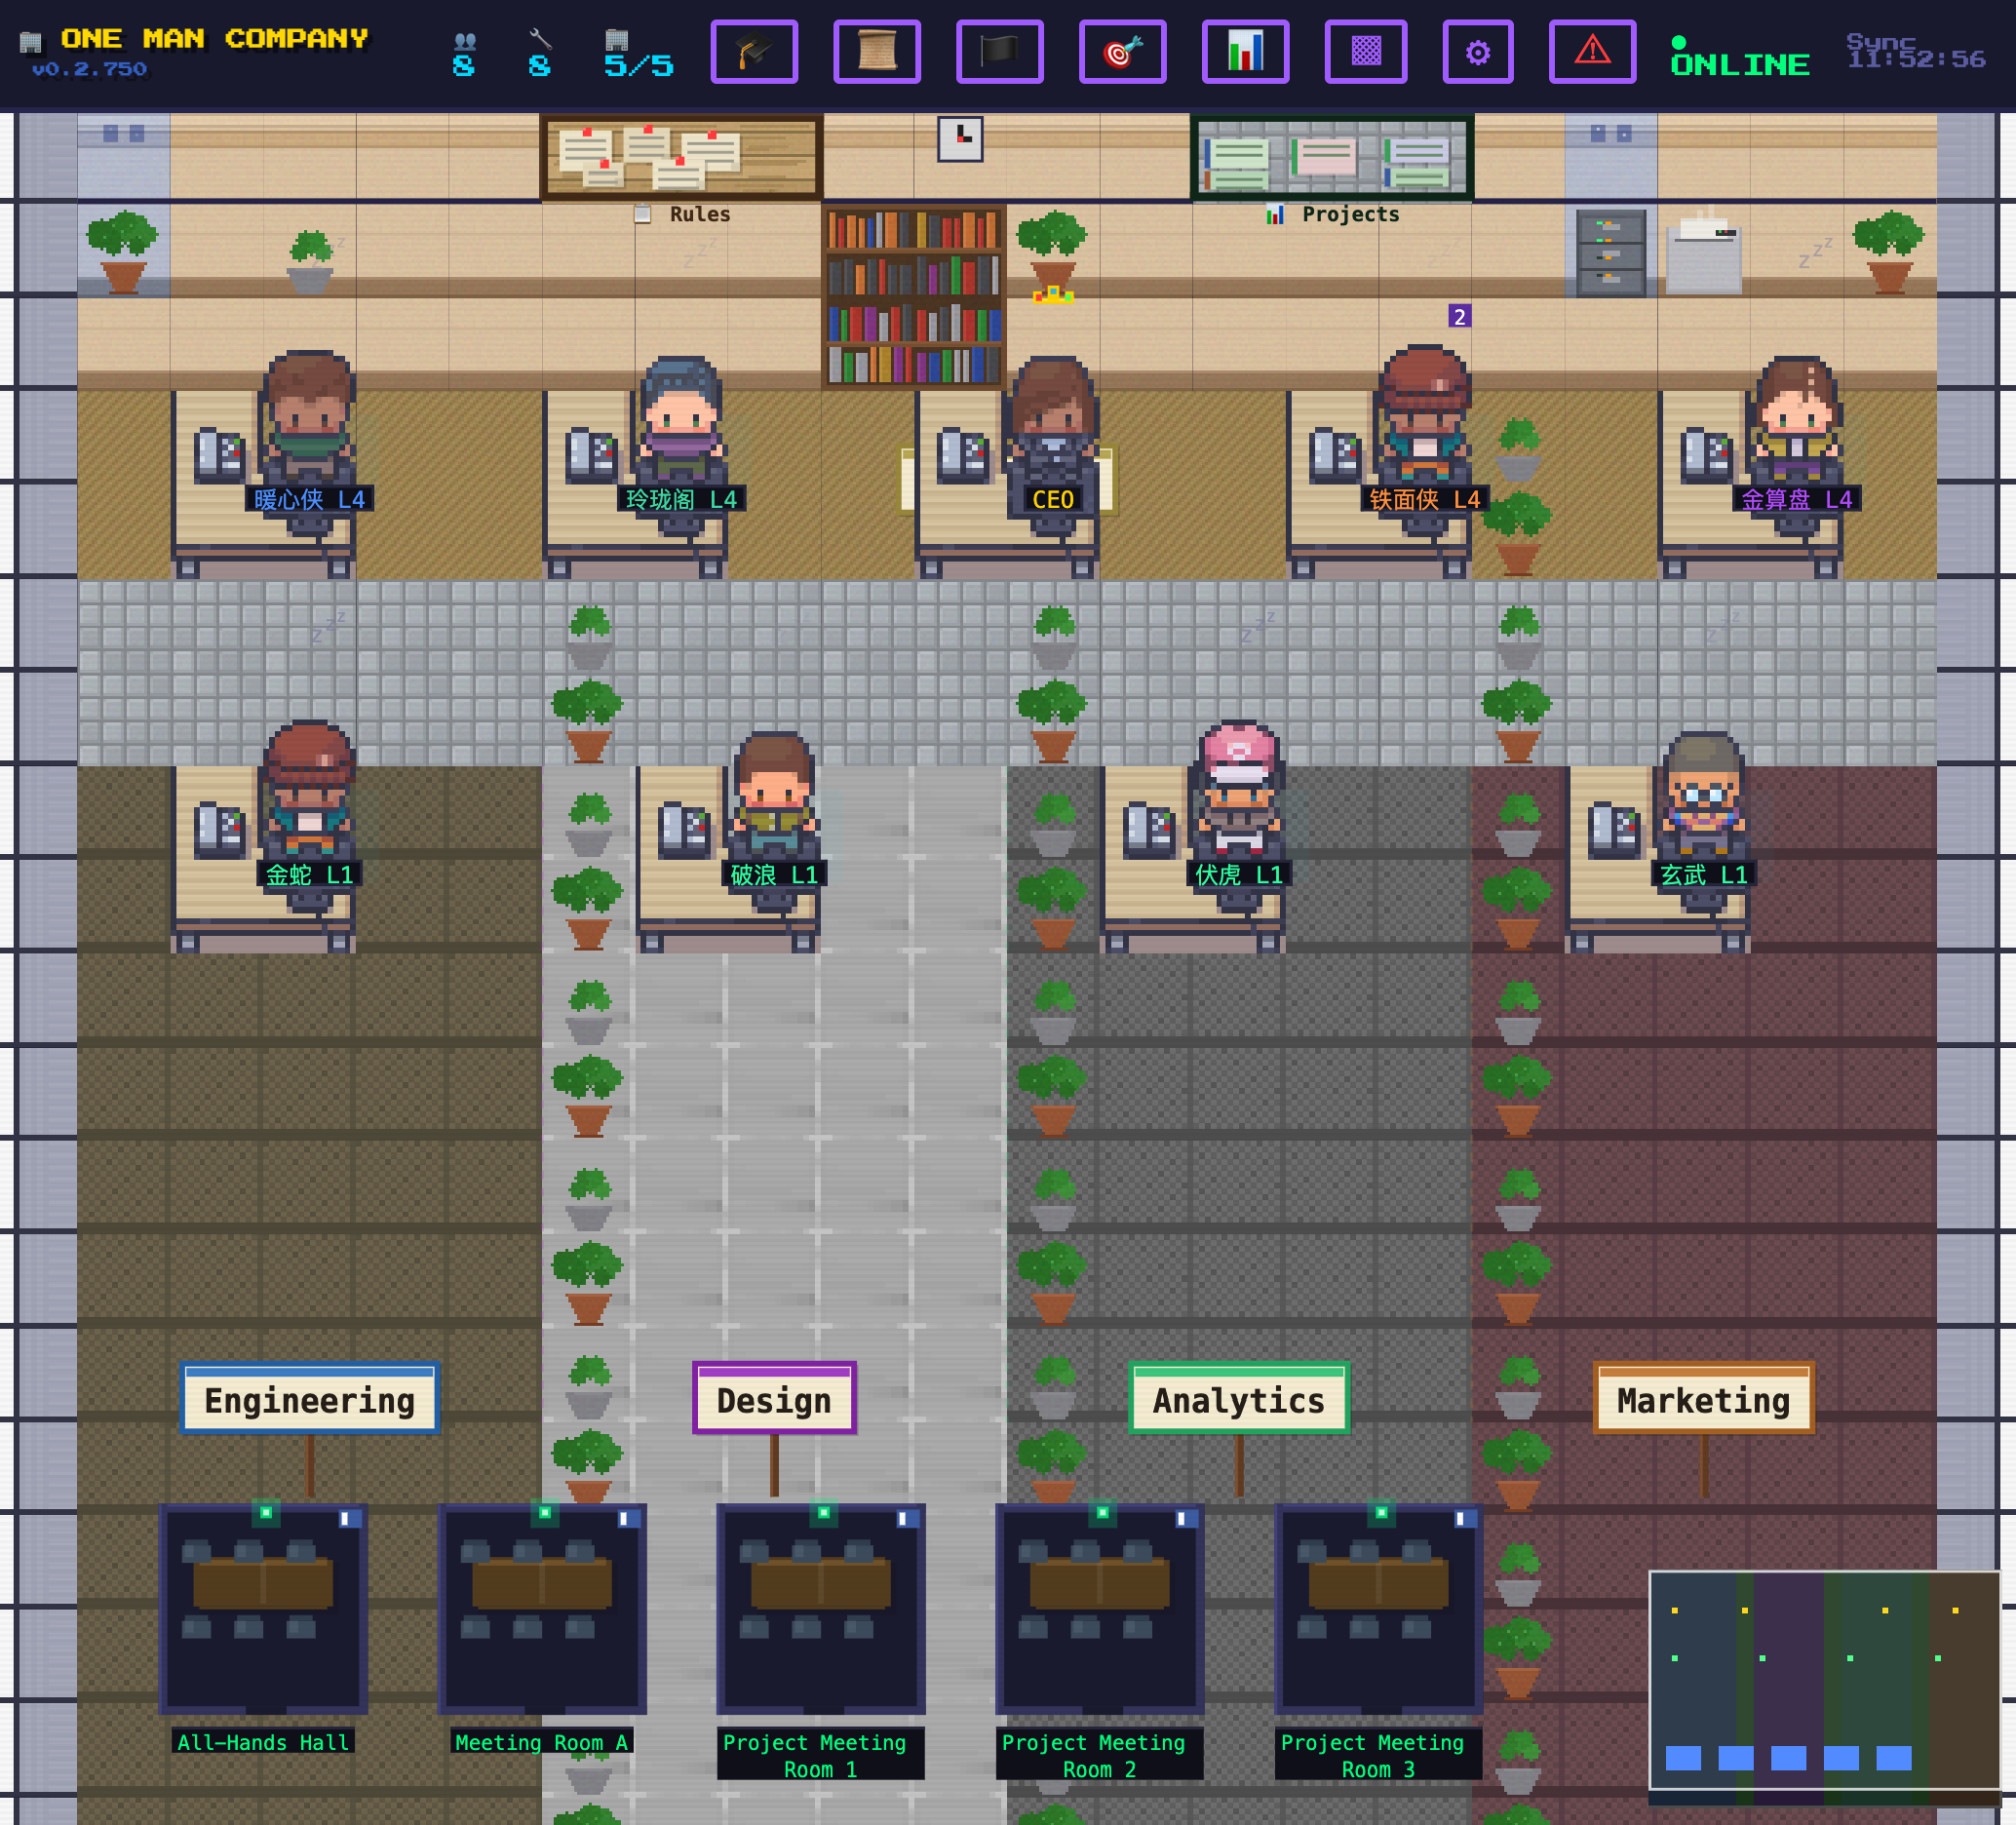
\includegraphics[width=\textwidth]{vide_1.png}\\
    \vspace{2pt}
    {\small(a) Assembled team workspace}
    \vspace{6pt}
    \includegraphics[width=\textwidth]{vide_6.png}\\
    \vspace{2pt}
    {\small(e) Generated scene: Polly Gray}
\end{minipage}
\hfill
\begin{minipage}[t]{0.30\textwidth}
    \vspace{0pt}
    \centering
    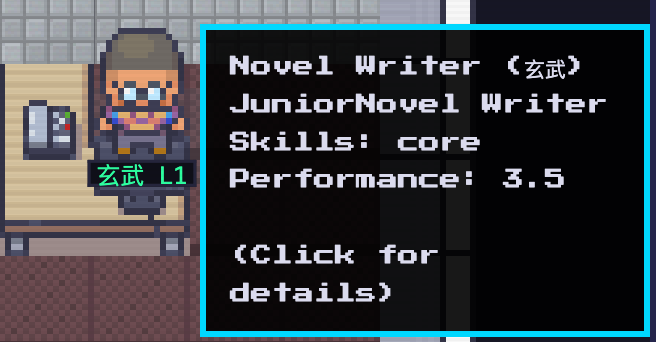
\includegraphics[width=\textwidth]{vide_2.png}\\
    \vspace{2pt}
    {\small(b) Novel Writer AI Agent}
    \vspace{6pt}
    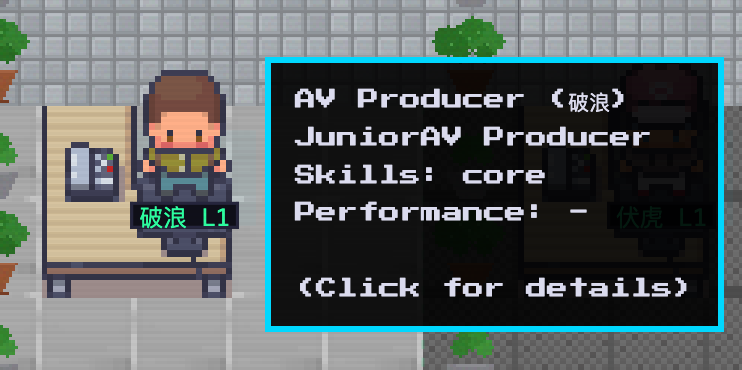
\includegraphics[width=\textwidth]{vide_3.png}\\
    \vspace{2pt}
    {\small(c) AV Producer AI Agent}
    \vspace{6pt}
    \includegraphics[width=\textwidth]{vide_7.png}\\
    \vspace{2pt}
    {\small(f) Generated scene: the raid}
\end{minipage}
\hfill
\begin{minipage}[t]{0.30\textwidth}
    \vspace{0pt}
    \centering
    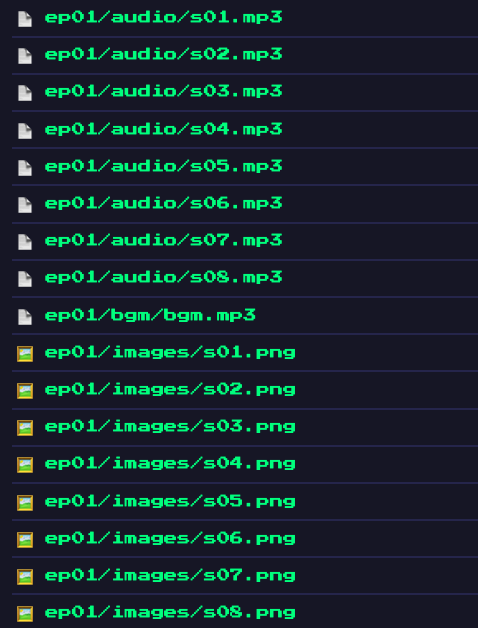
\includegraphics[width=\textwidth]{vide_4.png}\\
    \vspace{2pt}
    {\small(d) Project output artifacts}
    \vspace{6pt}
    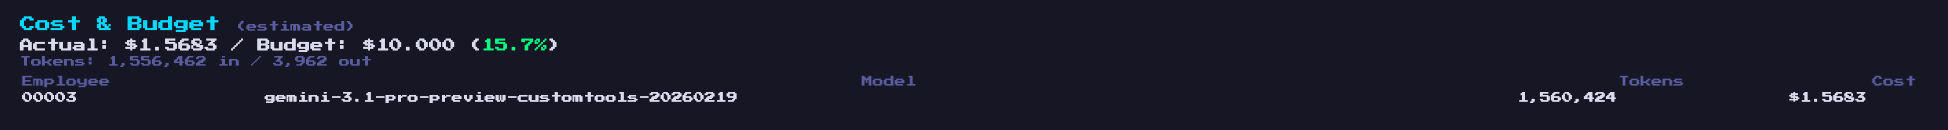
\includegraphics[width=\textwidth]{vide_5.png}\\
    \vspace{2pt}
    {\small(h) Cost \& token breakdown}
    \vspace{6pt}
    \includegraphics[width=\textwidth]{vide_8.png}\\
    \vspace{2pt}
    {\small(g) Generated scene: the racecourse}
\end{minipage}
\caption{
    \textbf{AI short drama case study: team assembly, recruited agents, generated scenes, and cost breakdown.}
    (a)~Company workspace after team assembly.
    (b)--(c)~Profile cards of the two recruited Talents.
    (d)~Output artifacts including episode scripts, scene images, voice-over audio, and final videos.
    (e)--(g)~Sample frames from the generated audiobook video, depicting animal-character scenes with narration overlays.
    (h)~Cost breakdown: approximately 1.56M tokens at \$1.57 total (15.7\% of the \$10 budget).
}
\label{fig:case-drama}
\end{figure}


The final output follows a modular directory structure, comprising sequentially generated scene images, voice-over tracks, background music, and a compiled video for each episode, alongside reusable execution scripts and verification logs. 
This case study highlights cross-modal coordination (text and audio-visual agents collaborating via a shared task tree), tool-augmented generation (the AV producer uses custom tools for image synthesis and text-to-speech), and cost efficiency (\$1.57 for 16 scenes, 16 voice-over tracks, background music, and two final videos).

\subsubsection{Automated Research Survey}

We demonstrate OMC's ability to conduct autonomous academic research through a survey task on world models for embodied AI and robotics.  The CEO provides a single prompt in Chinese:

\begin{mdframed}[
  nobreak=true,
  linewidth=0.8pt,
  linecolor=black!40,
  backgroundcolor=black!2,
  innertopmargin=10pt,
  innerbottommargin=10pt,
  innerleftmargin=14pt,
  innerrightmargin=14pt,
  roundcorner=4pt
]
\sloppy
\noindent\texttt{Survey the topic ``world models for embodied AI and robotics'' (2021--2026).  Produce a detailed, well-cited mind map and propose three feasible research ideas with descriptions.}
\end{mdframed}

\begin{figure}[H]
\centering
%% Row 1: workspace + output documents
\begin{minipage}[b]{0.52\textwidth}
    \centering
    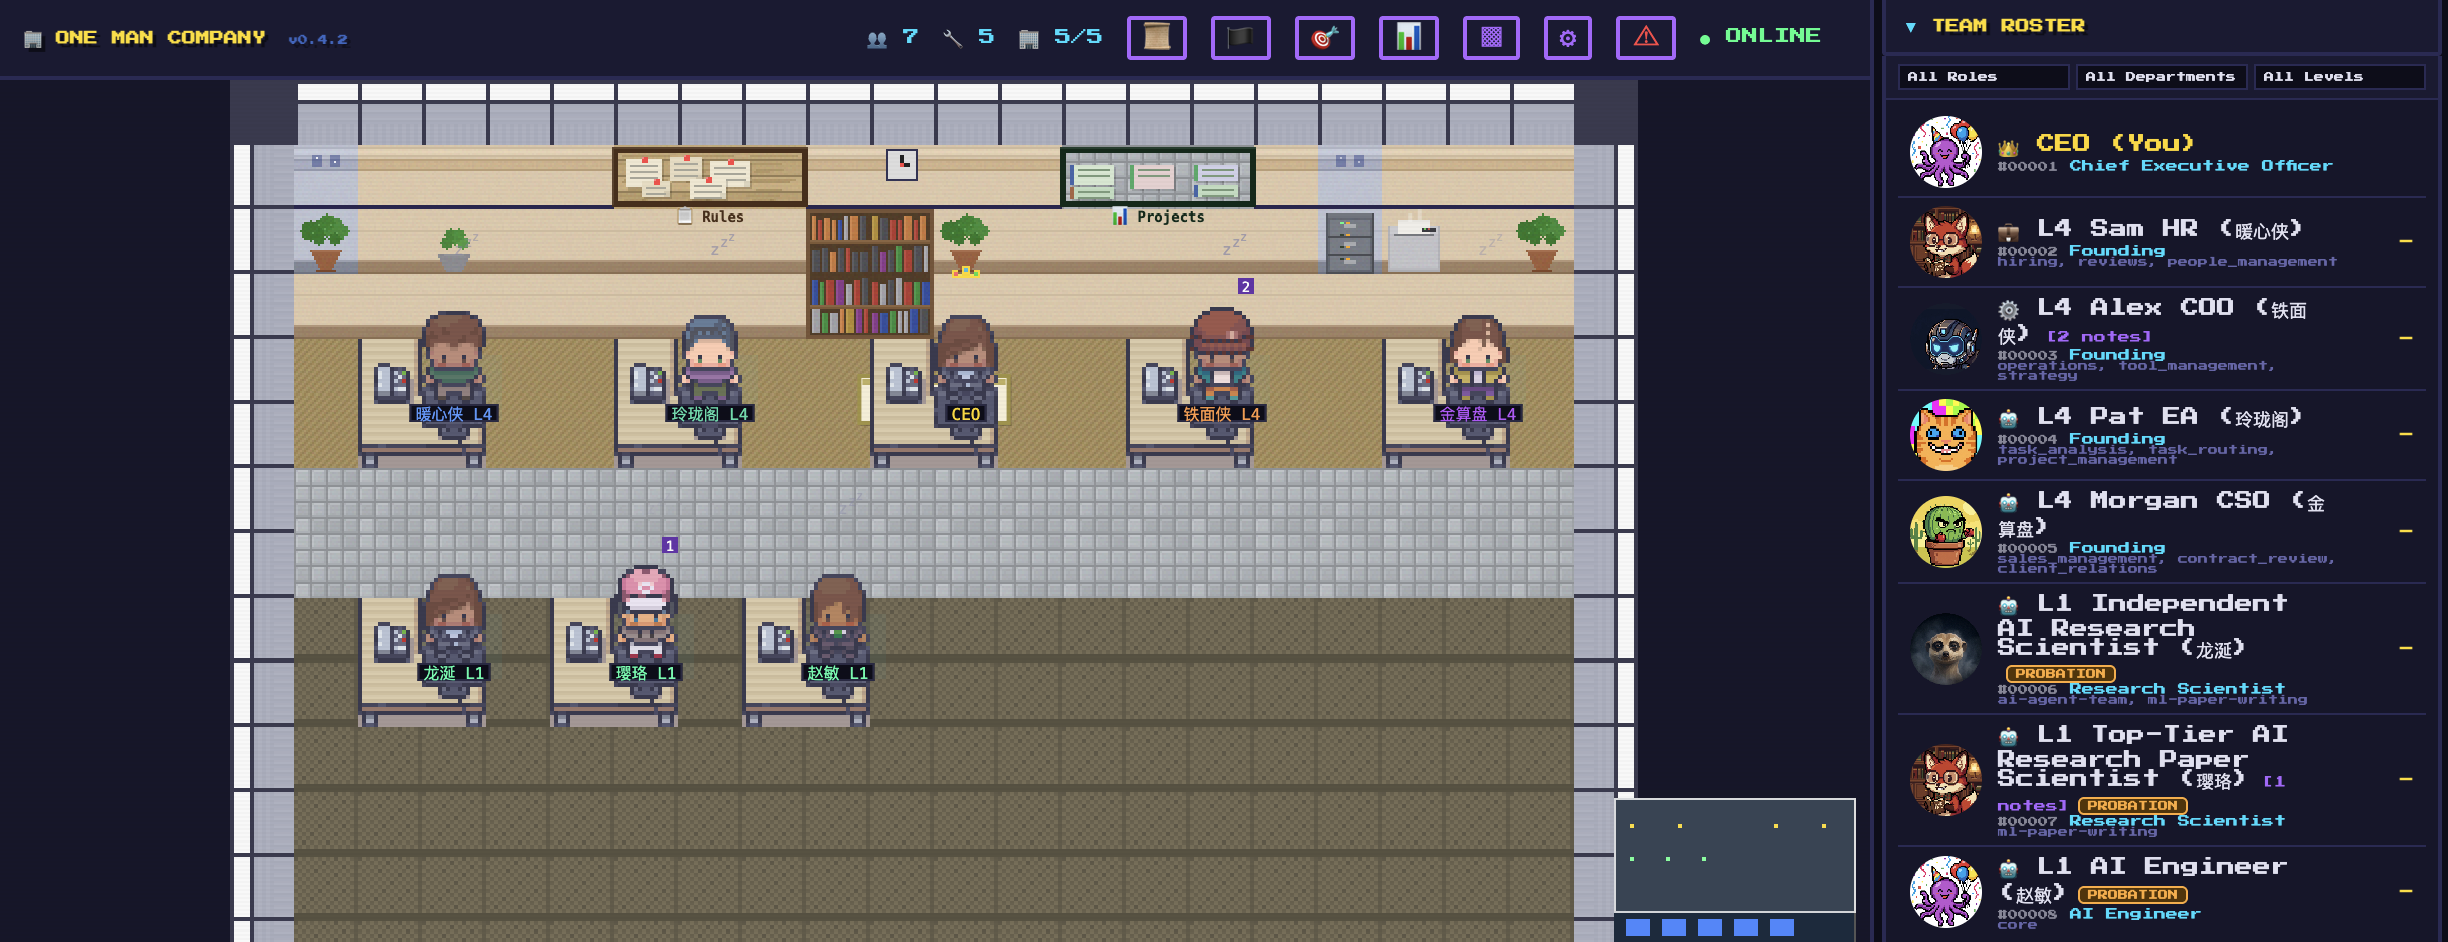
\includegraphics[width=\textwidth]{case4/all_agents.png}\\
    \vspace{2pt}
    {\small(a) Assembled research team}
\end{minipage}
\hfill
\begin{minipage}[b]{0.44\textwidth}
    \centering
    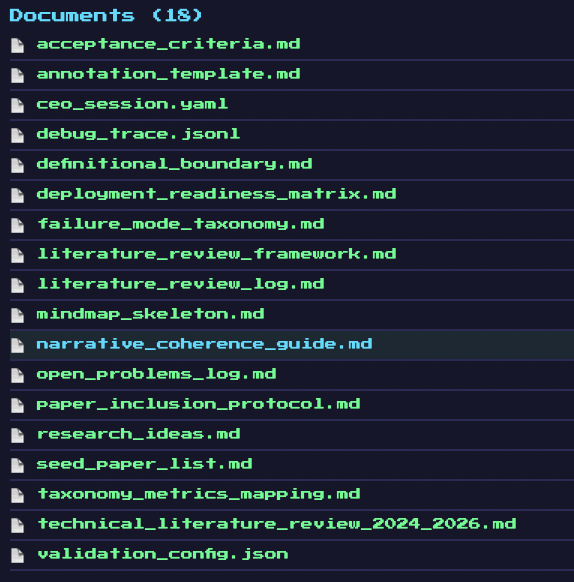
\includegraphics[width=\textwidth]{case4/filelist.png}\\
    \vspace{2pt}
    {\small(e) 18 output documents}
\end{minipage}

\vspace{8pt}

%% Row 2: agent profiles + cost
\begin{minipage}[b]{0.24\textwidth}
    \centering
    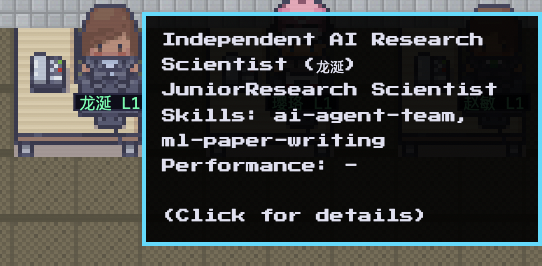
\includegraphics[width=\textwidth]{case4/reseascher_1.png}\\
    \vspace{2pt}
    {\small(b) Research Scientist}
\end{minipage}
\hfill
\begin{minipage}[b]{0.24\textwidth}
    \centering
    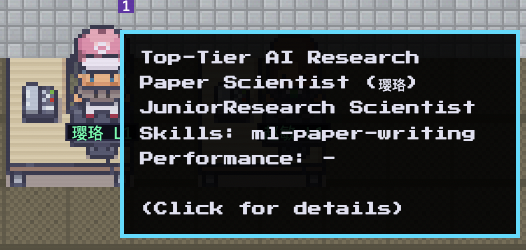
\includegraphics[width=\textwidth]{case4/reseascher_2.png}\\
    \vspace{2pt}
    {\small(c) Research Paper Scientist}
\end{minipage}
\hfill
\begin{minipage}[b]{0.24\textwidth}
    \centering
    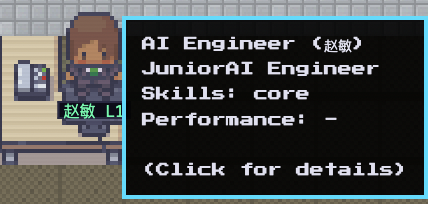
\includegraphics[width=\textwidth]{case4/engineer_1.png}\\
    \vspace{2pt}
    {\small(d) AI Engineer}
\end{minipage}
\hfill
\begin{minipage}[b]{0.24\textwidth}
    \centering
    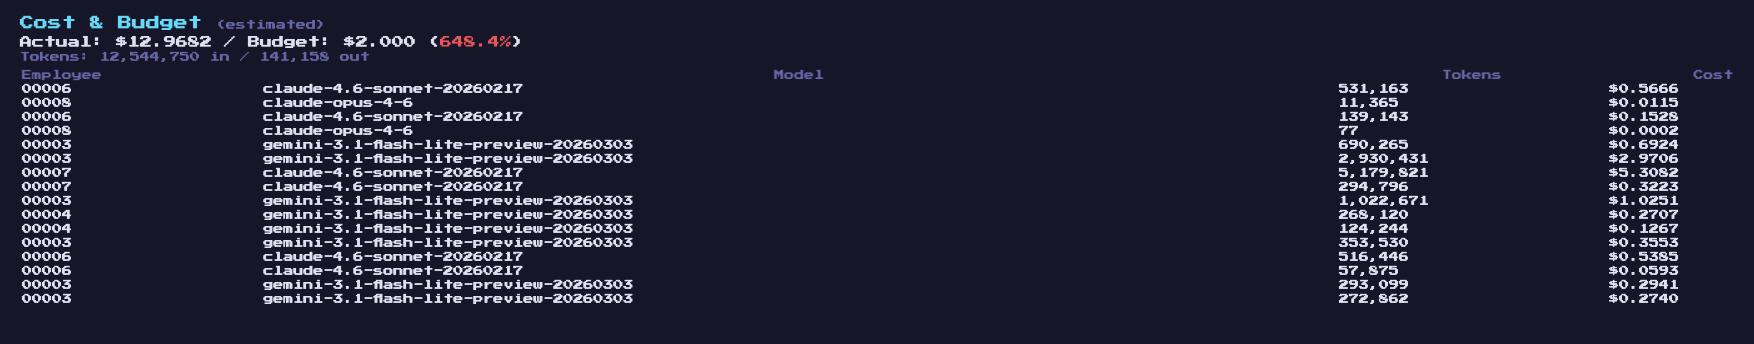
\includegraphics[width=\textwidth]{case4/cost.png}\\
    \vspace{2pt}
    {\small(f) Cost \& token breakdown}
\end{minipage}

\caption{
    \textbf{Automated research survey case study.}
    (a)~The OMC workspace after team assembly, with three recruited specialists seated alongside the founding team.
    (b)--(d)~Profile cards of the recruited Talents: two Research Scientists (Claude Sonnet~4.6) and one AI Engineer (self-hosted).
    (e)~The 18 deliverable documents produced autonomously, including literature reviews, failure mode taxonomies, and research proposals.
    (f)~Cost and token breakdown: \$16.26 total across 15.9M tokens.
}
\label{fig:case-research}
\end{figure}

The HR agent recruits three domain specialists from the Talent Market: a \textbf{Research Scientist} (Claude Sonnet~4.6) responsible for literature review and idea generation, a \textbf{Research Paper Scientist} (Claude Sonnet~4.6) for survey structure and documentation, and an \textbf{AI Engineer} (self-hosted) for technical benchmarking (Figure~\ref{fig:case-research}).  The COO decomposes the project into two phases.  In Phase~1, the three specialists work in parallel: one builds the survey skeleton, acceptance criteria, and a seed list of 35 papers; one reviews 17 papers and catalogues 8 open problems with 11 failure modes; and one benchmarks deployment readiness across 28 systems.  In Phase~2, the team produces a paper inclusion protocol, a 931-line literature review framework, and finally three novel research ideas grounded in the failure modes discovered in Phase~1.

The project completes in under two hours at a total cost of \$16.26 (15.9M tokens).  Deliverables include 17 structured documents, a rendered mind map covering six research themes with approximately 70 nodes (Appendix~\ref{sec:research-mindmap}), and three research proposals grounded in the failure modes discovered during the survey:

\begin{table}[H]
\centering
\caption{Research ideas generated autonomously by OMC from the world models survey.}
\label{tab:research-ideas}
\small
\setlength{\tabcolsep}{3pt}
\begin{tabularx}{\textwidth}{@{}>{\raggedright\arraybackslash}p{2.8cm}>{\raggedright\arraybackslash}p{3.5cm}>{\raggedright\arraybackslash}p{2.2cm}X@{}}
\toprule
\textbf{Idea} & \textbf{Problem Addressed} & \textbf{Target Venue} & \textbf{Key Technique} \\
\midrule
HiTeWM & Compounding prediction error beyond 15 steps & NeurIPS / ICLR & Two-level (fast 50Hz + slow 2Hz) architecture with uncertainty-gated re-grounding \\
\addlinespace
PhysWM & Physical implausibility in video-based WMs & ICML / CoRL & Differentiable physics constraints injected into latent dynamics \\
\addlinespace
MAWM & Sim-to-real domain shift + overconfident hallucination & CoRL / ICLR & Meta-learning across sim domains + conformal prediction for calibrated uncertainty \\
\bottomrule
\end{tabularx}
\end{table}

\noindent Each idea includes a technical formulation, expected baselines, and a 2--3 year research timeline (full details in Appendix~\ref{sec:research-ideas}).  We manually verified the quality of these outputs: all cited papers are real, the failure mode taxonomy is well-structured, and the third idea (MAWM, combining meta-learning with conformal prediction for sim-to-real transfer) has genuine novelty.  These results were produced in a single zero-shot iteration; with human review and subsequent iterations, the quality of both the survey coverage and research ideas can be further improved.  The entire pipeline, from a one-sentence brief to a complete survey with actionable research directions, runs without human intervention beyond the initial prompt.

Across all four case studies, the same pattern holds: the CEO provides a one-sentence brief, OMC recruits the right specialists, decomposes the project, executes it across heterogeneous backends, and delivers results, all without domain-specific configuration.  The content generation task used GPT-4o and Claude Sonnet~4; the game used Claude Sonnet~4 and Gemini~2.5; the audiobook used Gemini~3.1 Pro; the research survey used Claude Sonnet~4.6 and a self-hosted agent.  None required changes to the framework itself.


\section{Discussion}
\label{sec:discussion}

\paragraph{Limitations.}
Several limitations should be acknowledged.  First, our quantitative evaluation is confined to PRDBench (50 software development tasks); while the case studies demonstrate cross-domain applicability (content generation, game development, audiobook production, and academic research), systematic evaluation on non-coding benchmarks remains future work.  Second, the self-evolution mechanisms (one-on-ones, retrospectives, performance reviews) have been implemented and deployed but not yet quantitatively ablated; isolating the contribution of each mechanism requires longitudinal studies across many projects.  Third, the Harness abstraction introduces system complexity: maintaining six typed interfaces and three Vessel backends increases the engineering surface, and misconfigurations can produce subtle failures.  Fourth, OMC inherits the context window limitations of its underlying foundation models; long-running projects may exceed memory fidelity, and the current mitigation (progress logs, summarised histories) is approximate.  
\paragraph{Cost--performance trade-off.}
OMC's multi-agent coordination incurs significant cost overhead (approximately \$6.91 per PRDBench task).  This cost is justified for complex, project-level tasks where correctness matters more than token efficiency, but may not be appropriate for simple, single-turn queries.  A natural extension is adaptive dispatch: routing simple tasks to a single agent and reserving multi-agent coordination for tasks that exceed a complexity threshold.

\paragraph{Broader implications.}
The human-enterprise analogy that motivates OMC is deliberately general: the pattern of manage--plan--hire--learn applies to any domain, not just software development.  The case studies (content generation, game development, audiobook production) provide initial evidence of this generality.  We believe that as the Talent Market grows and more agent families become available, the organisational layer will become increasingly valuable, just as operating systems became more valuable as hardware diversity increased.


\section{Conclusion}
\label{sec:conclusion}

OMC shows that the organizational machinery of human companies (typed contracts between employees and the platform, structured task decomposition with review gates, on-demand recruitment, and performance-driven evolution) transfers to multi-agent coordination.  The Harness makes heterogeneous backends interchangeable; the Explore-Execute-Review loop decomposes and executes projects; the Talent Market grounds agent capabilities in tested artefacts; and the self-evolution pipeline ensures that agents and the organisation improve over time.  On PRDBench, this combination yields an 84.67\% success rate, surpassing all baselines, across projects that span multiple domains and require long-horizon reasoning.  The main open questions are whether this advantage holds at larger scale, how much each component contributes in isolation, and how the Talent Market ecosystem should grow to cover domains beyond software development.

% =====================================================================
\clearpage
\bibliographystyle{IEEEtran}
\bibliography{refs}
\clearpage
\appendix
\section*{Appendix}
\addcontentsline{toc}{section}{Appendix}



\section{Organisational Interface Signatures}
\label{sec:harness-signatures}

\begin{table}[H]
\centering
\caption{Organisational interface signatures.}
\label{tab:harness-interfaces}
\small
\setlength{\tabcolsep}{4pt}
\begin{tabularx}{\textwidth}{@{}>{\ttfamily\raggedright\arraybackslash}p{0.16\textwidth}>{\raggedright\arraybackslash}p{0.38\textwidth}X@{}}
\toprule
\textbf{Interface} & \textbf{Signature} & \textbf{Responsibility} \\
\midrule
Execution & \texttt{execute(task, ctx) $\to$ (result, cost)} & Dispatch task to backend, return output \\
\addlinespace
Task & \texttt{enqueue(task); dequeue() $\to$ task} & Per-employee queue, mutual exclusion \\
\addlinespace
Event & \texttt{publish(event); subscribe(filter)} & Organisational event bus \\
\addlinespace
Storage & \texttt{read(key) $\to$ data; write(key, data)} & Persistent memory (short/medium-term) \\
\addlinespace
Context & \texttt{assemble(role, guidance, memory) $\to$ ctx} & Execution context construction \\
\addlinespace
Lifecycle & \texttt{pre\_hook(task, ctx); post\_hook(task, result)} & Validation, guardrails, self-improvement \\
\bottomrule
\end{tabularx}
\end{table}

\section{Organisation Layer--OS Kernel Correspondence}
\label{sec:os-mapping}

The six organisational interfaces correspond to the canonical subsystems of an OS kernel as identified in standard references~\cite{tanenbaum2014modern, silberschatz2018os}.  Table~\ref{tab:os-correspondence} maps each kernel subsystem to the organisational interface(s) that fulfil the analogous role for agent workforces.

\begin{table}[H]
\centering
\caption{Mapping from classical OS kernel subsystems to OMC organisational interfaces.}
\label{tab:os-correspondence}
\small
\setlength{\tabcolsep}{4pt}
\begin{tabularx}{\textwidth}{@{}>{\raggedright\arraybackslash}p{0.17\textwidth}>{\raggedright\arraybackslash}p{0.20\textwidth}>{\ttfamily\raggedright\arraybackslash}p{0.14\textwidth}X@{}}
\toprule
\textbf{OS Subsystem} & \textbf{Kernel Responsibility} & \textbf{Org. Interface} & \textbf{OMC Realisation} \\
\midrule
Process Mgmt. & Create, schedule, and terminate processes & Execution, Task & Dispatch tasks to Containers; enforce mutual exclusion ($|\text{running}(e)| \leq 1$); manage per-employee task queues with enqueue/dequeue semantics \\
\addlinespace
Memory Mgmt. & Allocate address spaces; isolate process memory & Context & Assemble the execution context (role identity, working principles, accumulated memory) each agent sees at runtime \\
\addlinespace
File System & Persistent storage with uniform read/write API & Storage & Uniform \texttt{read}/\texttt{write} over heterogeneous backends (YAML profiles, progress logs, memory stores) \\
\addlinespace
I/O \& Device Mgmt. & Abstract heterogeneous hardware behind driver interfaces & Container contract & Each Container type implements the six organisational interfaces so the platform never touches backend-specific APIs \\
\addlinespace
IPC & Message passing, signals, shared memory & Event & Publish--subscribe event bus for organisational events across all agents \\
\addlinespace
Security \& Audit & Policy enforcement, access control, accounting & Lifecycle & Pre-task hooks enforce guardrails and input validation; post-task hooks perform self-reflection and audit logging \\
\bottomrule
\end{tabularx}
\end{table}


\section{Executor Backends and Task Dispatch}
\label{sec:execution}
% ─────────────────────────────────────────────────────────────────────

\paragraph{On-Demand Dispatch.}
Agents do not poll for work. Tasks are dispatched on demand: execution begins immediately through the organisational layer when a task is assigned, and the agent consumes no resources when idle. The system scales naturally---adding agents does not increase idle overhead---and recovers from interruptions because all state is persisted rather than held in running processes.

\paragraph{Three Reference Backends.}
The execution interface decouples task dispatch from the agent runtime. Three reference implementations are provided: (1)~a LangChain-based reactive agent for tool-using tasks, (2)~a Claude Code session for long-horizon reasoning, and (3)~a script-based executor for lightweight or custom runtimes. Because the organisational layer carries all state, each executor is kept stateless and minimal. Additional backends can be registered without changes to existing agents or infrastructure.

\paragraph{Failure Recovery.}
When an agent fails a task, the failure is captured, error context is injected into the retry prompt, and execution resumes with updated information. After a configurable number of attempts, the task is escalated to the supervising agent for review and reassignment. This recovery loop operates entirely through the organisational interfaces, so the behavior is consistent across executor backends.

% ─────────────────────────────────────────────────────────────────────
\subsection{Tool and Skill System}
\label{sec:tools}
% ─────────────────────────────────────────────────────────────────────

\paragraph{Role-Based Tool Access.}
An agent's action space is determined by which tools it is authorized to use. The system enforces this through a unified tool registry that gates access by role, explicit permission grants, and asset ownership. Permissions are resolved at prompt assembly time: each agent's context includes only authorized tools, so capability boundaries are enforced before the agent begins reasoning.

\begin{table}[H]
\centering
\caption{Tool permission categories}
\label{tab:tools}
\small
\setlength{\tabcolsep}{4pt}
\begin{tabularx}{\textwidth}{@{}>{\raggedright\arraybackslash}p{0.16\textwidth}>{\raggedright\arraybackslash}p{0.31\textwidth}X@{}}
\toprule
\textbf{Category} & \textbf{Access Rule} & \textbf{Examples} \\
\midrule
Base & All employees & \texttt{dispatch\_child}, \texttt{accept\_child}, \texttt{read\_file} \\
Gated & Requires \texttt{tool\_permissions} in profile & Email integration, external API access \\
Role & Employee role $\in$ \texttt{allowed\_roles} & \texttt{code\_review} (Reviewer), design tools (Designer) \\
Asset & \texttt{allowed\_users} includes employee ID & Company-specific tools, Talent-provided tools \\
\bottomrule
\end{tabularx}
\end{table}

\paragraph{Cross-Backend Tool Exposure.}
Tools are exposed through a standard interface regardless of executor backend. For Claude Code sessions, tools are surfaced via the Model Context Protocol (MCP), allowing the same organizational capabilities as LangChain-based agents. From the platform perspective, MCP bridging is an implementation detail of one executor---the tool contract is uniform across backends.

\paragraph{Tools as Inter-Agent Coordination.}
Core inter-agent tools cover the full range of organizational interaction: delegating work to a subordinate, accepting or rejecting a subtask, convening a multi-agent discussion, and escalating a decision to the CEO. Each interaction is expressed as a tool call that flows through the organisational layer and produces effects visible to all agents.

\section{Talent Market: A Three-Type Agent Supply Chain}
\label{sec:talent-supply}
% ─────────────────────────────────────────────────────────────────────

The Talent Market is the supply-side complement to the Container abstraction: while the Container defines \emph{how} an agent executes, the Talent Market determines \emph{what} cognitive capability is available for hire. It provides three types of agent sourcing, each representing a different method of constructing a Talent package. The three types are not ranked by quality or priority---they are parallel supply channels, and all produce standard Talent packages that enter the OMC runtime through the same pathway: loaded into a Container and governed by the organisational interfaces. Once hired, every agent begins at the same employee level regardless of its sourcing type.

\paragraph{Type 1: Curated Repository Agents.}
Type~1 agents are manually packaged from established open-source agent repositories. Each source project is selected based on community adoption metrics and benchmark performance; its core reasoning strategies, tool interfaces, and domain knowledge are distilled into the OMC Talent package format, stripping framework-specific runtime dependencies. The resulting Talents are validated against reference tasks to ensure behavioral fidelity. This sourcing method is best suited for domains where mature, battle-tested agent implementations already exist in the open-source ecosystem.

\paragraph{Type 2: Prompt-Sourced Agents with Skill Assembly.}
Type~2 agents start from high-quality \emph{system prompts} sourced from community-curated prompt repositories---notably the Agency-Agents collection~\cite{agencyagents}, which provides over 140 specialist personas spanning engineering, design, marketing, product, sales, project management, testing, and other divisions. Each persona defines a detailed identity, working principles, deliverable specifications, and success metrics, but carries no executable tool bindings or runtime skills. To transform a persona into a deployable Talent, OMC applies an automated \textbf{skill assembly} step: the system queries the SkillsMP marketplace~\cite{skillsmp} using the persona’s domain descriptors and capability requirements as a structured search query, retrieves compatible skills (tool bindings, behavioral principles, workflow fragments), and composes them with the source persona into a complete Talent package. This sourcing method is best suited when a well-defined role description exists but no complete agent implementation is available.

\paragraph{Type 3: Dynamic Agent Assembly from Cloud Skills.}
Type~3 agents are assembled entirely from modular skills retrieved from SkillsMP~\cite{skillsmp}, an open community-driven skill marketplace that aggregates agent skills from public GitHub repositories using the standardized \texttt{SKILL.md} format. Unlike Type~1 (which packages an existing implementation) or Type~2 (which starts from a curated persona), Type~3 constructs \emph{both} the persona and the skill set on demand. The HR agent provides a structured job description based on the task specification; the Talent Market then performs semantic search over skill metadata, filters for mutual compatibility and interface compliance, ranks by relevance and community score, and synthesizes a coherent agent identity from the retrieved components. This sourcing method is best suited for niche or emerging domains where neither complete agent implementations nor established persona templates yet exist, and also serves as a \emph{cold-start} mechanism for the Talent Market as a whole.

\paragraph{Human-in-the-Loop Talent Selection.}
Talent hiring is not fully automated: the system presents a ranked \emph{top-$k$} recommendation list to the CEO, who makes the final selection. To ensure the CEO sees a diverse range of sourcing methods, the recommendation engine composes the shortlist with an approximately 80/20 distribution---roughly 80\% of candidates from Type~1 and Type~2, and 20\% from Type~3. This ratio reflects the current relative maturity of each supply channel rather than an intrinsic quality ordering: Type~1 and Type~2 draw from repositories with established community validation, while Type~3’s dynamically assembled agents offer broader coverage but have not undergone prior community review. The CEO can inspect each candidate’s provenance---source repository for Type~1, source persona and attached skills for Type~2, constituent skills for Type~3---and approve or reject before the hiring pipeline provisions a Container.

\paragraph{Cross-Type Feedback.}
The three sourcing channels are not isolated: skills refined through deployed agents’ self-improving loops can be published back to the skill marketplace, enriching the community pool regardless of which type originally produced the agent. Similarly, a Type~3 agent whose synthesized persona proves effective across multiple projects can have that persona persisted and contributed to prompt repositories, expanding the available pool for future Type~2 sourcing.


\section{Case 1: GitHub AI Agent Weekly Trend Report}
\label{appendix:github-report}

\begin{figure}[H]
\centering
\begin{minipage}[c]{0.30\textwidth}
    \centering
    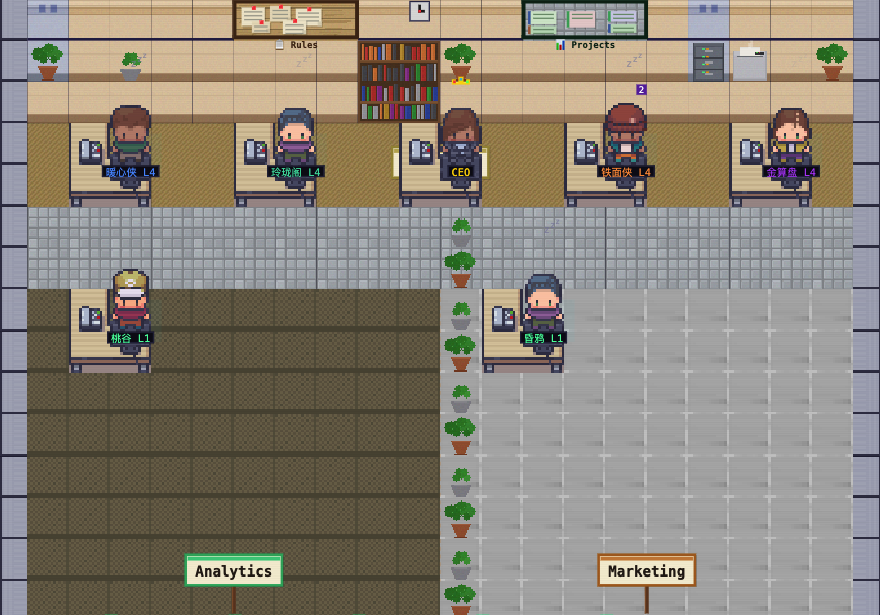
\includegraphics[width=\textwidth]{news-team.png}\\
    \vspace{2pt}
    {\small(a) Assembled team workspace}
\end{minipage}
\hfill
\begin{minipage}[c]{0.28\textwidth}
    \centering
    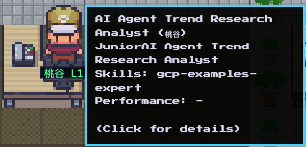
\includegraphics[width=\textwidth]{trend-researcher.png}\\
    \vspace{2pt}
    {\small(b) AI Agent Trend Research Analyst}

    \vspace{8pt}

    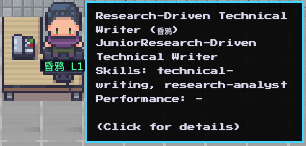
\includegraphics[width=\textwidth]{writer-2.png}\\
    \vspace{2pt}
    {\small(c) Research-Driven Technical Writer}
\end{minipage}
\hfill
\begin{minipage}[c]{0.36\textwidth}
    \centering
    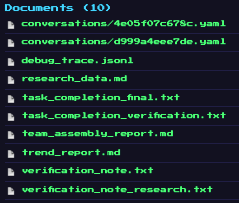
\includegraphics[width=\textwidth]{materials.png}\\
    \vspace{2pt}
    {\small(d) Project output documents}

    \vspace{8pt}

    
\includegraphics[width=\textwidth]{cost.png}\\
    \vspace{2pt}
    {\small(e) Cost \& token breakdown}
\end{minipage}

\caption{
    \textbf{Content-generation case study: team assembly, recruited agents, output artefacts, and cost breakdown.}
    (a) The OMC company workspace after team assembly, with the newly hired agents (L1) seated in the Analytics and Marketing departments.
    (b)--(c) Profile cards of the two recruited Talents: an AI Agent Trend Research Analyst and a Research-Driven Technical Writer.
    (d) Project documents produced autonomously, including \texttt{research\_data.md}, \texttt{trend\_report.md}, and verification logs.
    (e) Cost and token usage breakdown across all participating employees, totalling \$4.49.
}
\label{fig:case-content}
\end{figure}

The following report was autonomously produced by the Writer agent (Claude Sonnet~4)
in the content-generation case study (Section~\ref{sec:case-content}), based on
research data collected by the Researcher agent (GPT-4o) and subsequently emailed
to the CEO without human editing.

\begin{mdframed}[
  linewidth=0.8pt,
  linecolor=black!40,
  backgroundcolor=black!2,
  innertopmargin=16pt,
  innerbottommargin=16pt,
  innerleftmargin=18pt,
  innerrightmargin=18pt,
  roundcorner=4pt
]
\sloppy
{\centering
  {\large\bfseries GitHub AI Agent Trending Repositories Report}\\[4pt]
  {\normalsize\bfseries Past Week Analysis (March 18--25, 2026)}\\[2pt]
  \textit{\small Researcher: GPT-4o\quad|\quad Writer: Claude Sonnet~4\quad|\quad Generated: March 25, 2026}
\par}

\vspace{8pt}
\hrule height 0.4pt
\vspace{10pt}

\noindent\textbf{Executive Summary}

\noindent
This comprehensive report analyzes the most significant AI Agent repositories that gained traction on GitHub during the past week (March 18--25, 2026). Our research identified 15 notable repositories spanning from enterprise-grade solutions to specialized domain applications, representing a total of over 4,000 stars across all projects.

\vspace{8pt}
\noindent\textbf{Key Market Trends}

\noindent\textit{Multi-Platform Integration Dominance.}\quad
The most significant trend is the surge in cross-platform agent integrations, particularly targeting Chinese market platforms: \textbf{weixin-agent-sdk} (887 stars) --- WeChat Clawbot integration; \textbf{astronclaw-tutorial} (268 stars) --- AstronClaw \& Loomy AI assistant tutorials.

\vspace{4pt}
\noindent\textit{Agent-to-Agent Communication Revolution.}\quad
A new paradigm is emerging with autonomous agent collaboration: \textbf{ClawLink} (246 stars) --- AI Agent Social Network enabling direct agent-to-agent communication; \textbf{HyperAgents} (784 stars) --- Self-referential self-improving agents.

\vspace{4pt}
\noindent\textit{Specialized Domain Applications.}\quad
Agents are becoming increasingly specialized: \textbf{app-store-preflight-skills} (936 stars) --- App Store compliance scanning; \textbf{ctf-agent} (194 stars) --- Autonomous CTF solver (1st place BSidesSF 2026); \textbf{buzz-bd-agent} (4 stars) --- Business development automation.

\vspace{8pt}
\noindent\textbf{Top Performing Repositories}

\vspace{4pt}
\noindent\textit{Most Popular (500+ Stars)}

\vspace{2pt}
\noindent\textbf{1.~app-store-preflight-skills} $\bigstar$~936\quad
\url{https://github.com/truongduy2611/app-store-preflight-skills}\\
AI agent skill for scanning iOS/macOS projects for App Store rejection patterns. Addresses a critical pain point for mobile developers.

\vspace{4pt}
\noindent\textbf{2.~weixin-agent-sdk} $\bigstar$~887\quad
\url{https://github.com/wong2/weixin-agent-sdk}\\
Clawbot WeChat integration for any Agent. Opens Chinese market access for global AI agents.

\vspace{4pt}
\noindent\textbf{3.~HyperAgents} $\bigstar$~784\quad
\url{https://github.com/facebookresearch/HyperAgents}\\
Self-referential self-improving agents for any computable task. Represents a breakthrough in autonomous self-improvement.

\vspace{6pt}
\noindent\textit{High Growth Projects (200--500 Stars)}

\vspace{2pt}
\noindent\textbf{4.~cc-skills-golang} $\bigstar$~281\quad \url{https://github.com/samber/cc-skills-golang}\quad Golang agentic skills collection.

\noindent\textbf{5.~astronclaw-tutorial} $\bigstar$~268\quad \url{https://github.com/iflytek/astronclaw-tutorial}\quad Complete tutorial for AstronClaw (cloud) \& Loomy (desktop) AI.

\noindent\textbf{6.~ClawLink} $\bigstar$~246\quad \url{https://github.com/CN-Syndra/ClawLink}\quad AI Agent Social Network for autonomous agent communication.

\noindent\textbf{7.~agent-kernel} $\bigstar$~226\quad \url{https://github.com/oguzbilgic/agent-kernel}\quad Minimal kernel for stateful AI coding agents.

\vspace{8pt}
\noindent\textbf{Emerging Innovation Areas}

\noindent\textit{Infrastructure \& Tooling}:\quad \textbf{usecomputer} (136 stars) --- Fast computer automation CLI; \textbf{agent-kanban} (22 stars) --- Mission control for AI workforce.

\noindent\textit{Security \& Compliance}:\quad \textbf{ctf-agent} (194 stars) --- Autonomous CTF solver; \textbf{copilot-cli-knowledge-agents} (2 stars) --- 13 specialized agents with security council.

\noindent\textit{Development Workflow}:\quad \textbf{spec\_driven\_develop} (189 stars) --- Spec-driven development; \textbf{flyai-skill} (171 stars) --- Alibaba's fly AI agent skill collection.

\hrule height 0.4pt

\noindent\textbf{Conclusion}\quad
The past week demonstrates accelerating innovation across platform integration (especially Chinese markets), agent autonomy (self-improvement and collaboration), enterprise applications, and infrastructure maturation. The total engagement of 4,000+ stars across 15 repositories indicates strong developer interest and continued rapid growth in the AI Agent ecosystem.

\noindent{\small\textit{Methodology: GitHub API~v4 queries targeting repositories created/updated March 18--25, 2026, keywords ``ai agent'', ``autonomous agent'', ``llm agent''. All links verified against GitHub trending algorithms. Total repositories analyzed: 50+.}}

\end{mdframed}
\newpage
\section{Case 2: Game Development}
\label{sec: game-dev}

\begin{figure}[H]
\centering
\begin{minipage}[c]{0.30\textwidth}
    \centering
    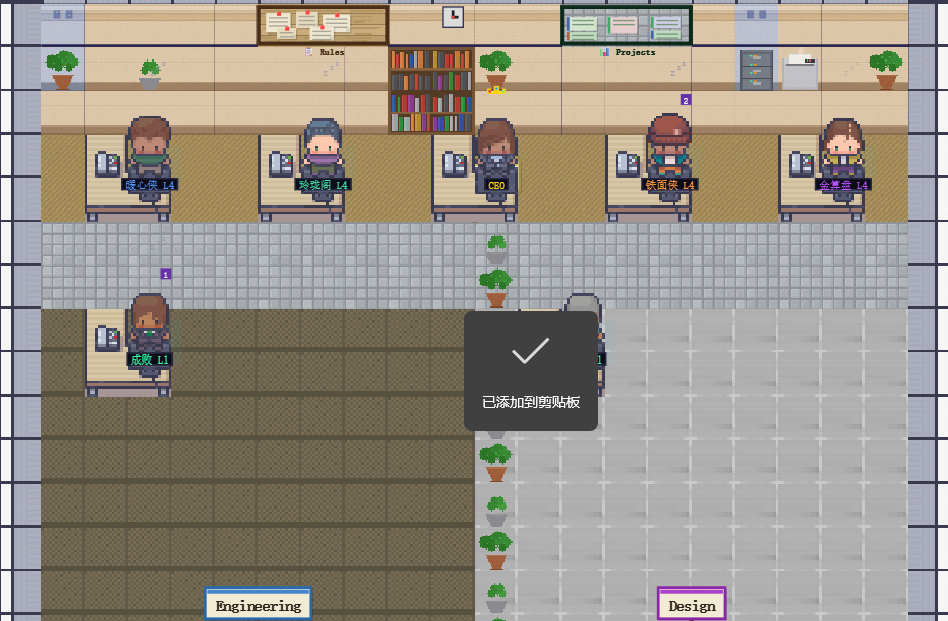
\includegraphics[width=\textwidth]{GAME-workflow/1.png}\\
    \vspace{2pt}
    {\small(a) Assembled team workspace}
    \vspace{8pt}
    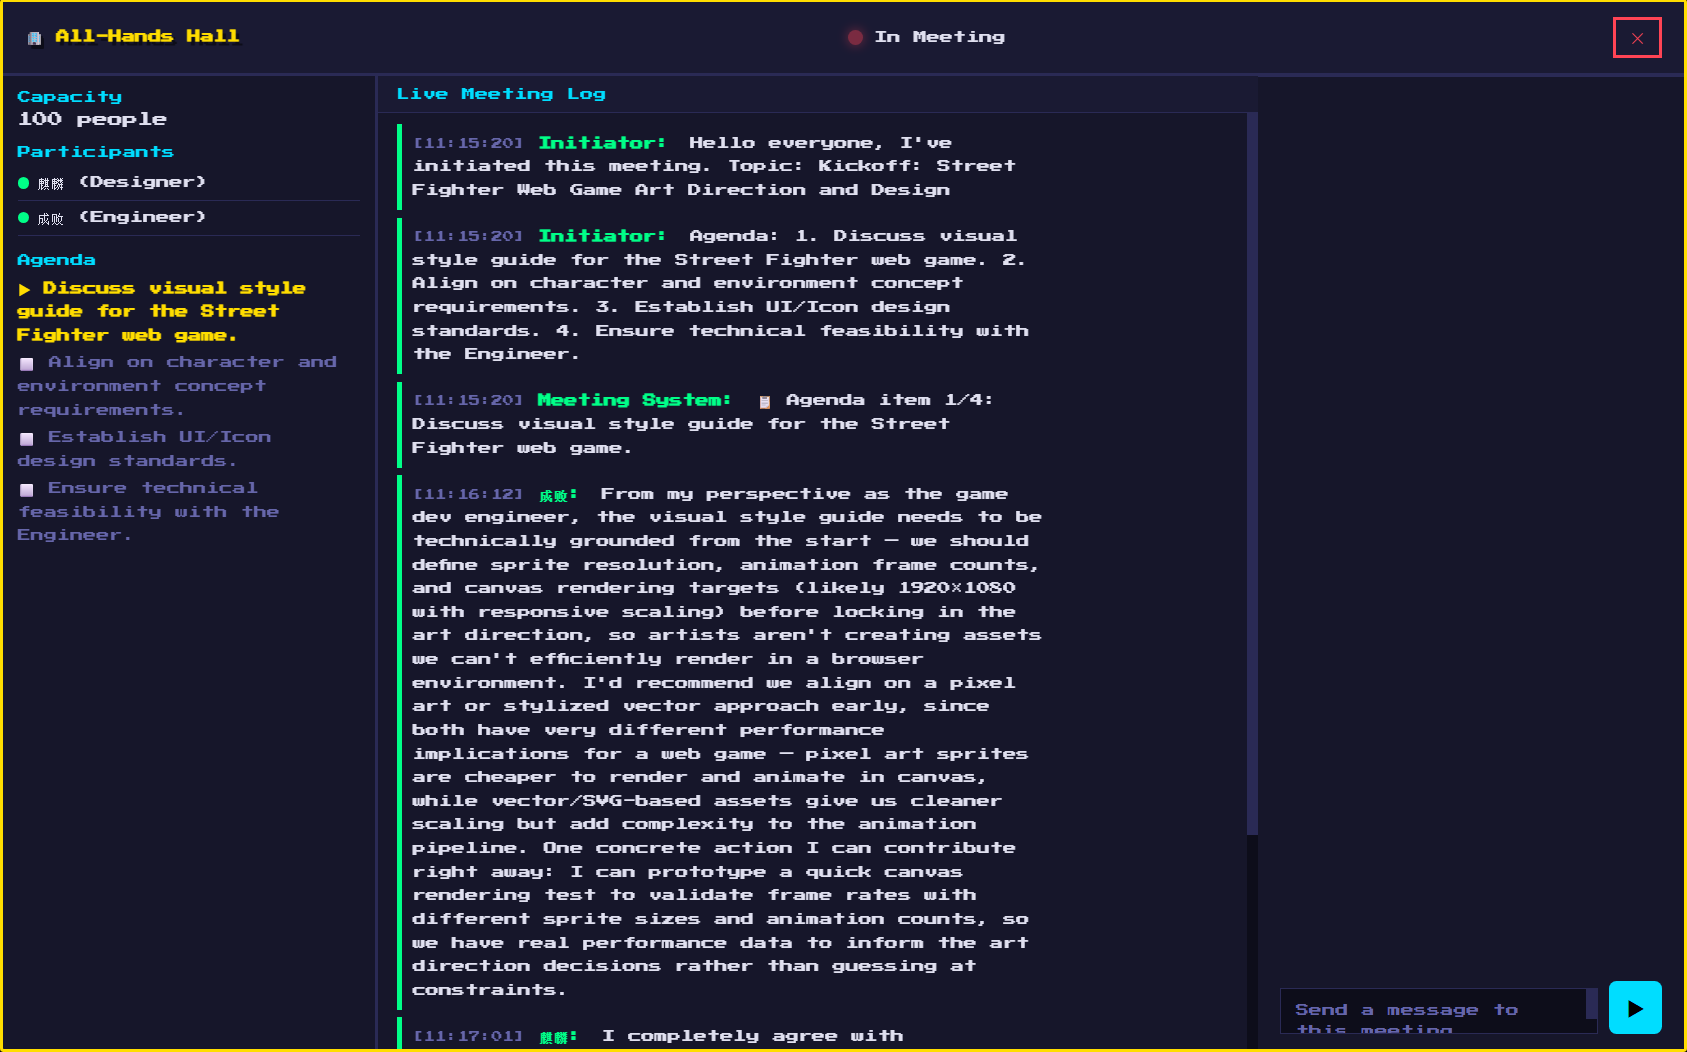
\includegraphics[width=\textwidth]{GAME-workflow/2.png}\\
    \vspace{2pt}
    {\small(b) Group meeting: Game Developer \& Art Designer}
\end{minipage}
\hfill
\begin{minipage}[c]{0.30\textwidth}
    \centering
    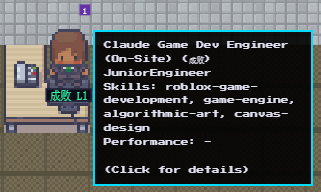
\includegraphics[width=\textwidth]{GAME-workflow/3.png}\\
    \vspace{2pt}
    {\small(c) Game Developer AI Agent}
    \vspace{8pt}
    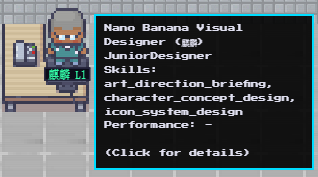
\includegraphics[width=\textwidth]{GAME-workflow/4.png}\\
    \vspace{2pt}
    {\small(d) Art Designer AI Agent}
\end{minipage}
\hfill
\begin{minipage}[c]{0.30\textwidth}
    \centering
    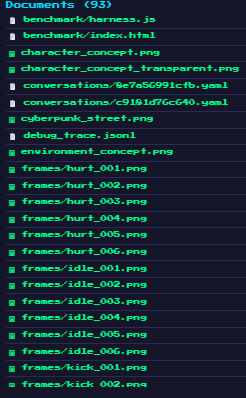
\includegraphics[width=\textwidth]{GAME-workflow/5.png}\\
    \vspace{2pt}
    {\small(e) Project output documents}
    \vspace{8pt}
    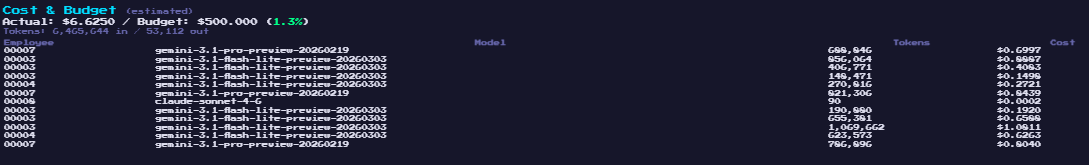
\includegraphics[width=\textwidth]{GAME-workflow/6.png}\\
    \vspace{2pt}
    {\small(f) Cost \& token breakdown}
\end{minipage}
\caption{
    \textbf{Street fight game case study: team assembly, recruited agents, output artefacts, and cost breakdown.}
    (a) The OMC company workspace after team assembly, with the newly hired agents (L1) seated in the Game Development and Art departments.
    (b) Group meeting between the Game Developer and Art Designer agents collaborating on game design.
    (c)--(d) Profile cards of the two recruited Talents: a Game Developer AI Agent and an Art Designer AI Agent.
    (e) Project documents produced autonomously, including \texttt{game\_design.md}, \texttt{asset\_list.md}, and verification logs.
    (f) Cost and token usage breakdown across all participating employees.
}
\label{fig:case-game}
\end{figure}

\newpage
\section{Case 3: Audio Book Development}
\label{sec: audio-book}

\begin{figure}[!htbp]
\centering
\begin{minipage}[c]{0.30\textwidth}
    \centering
    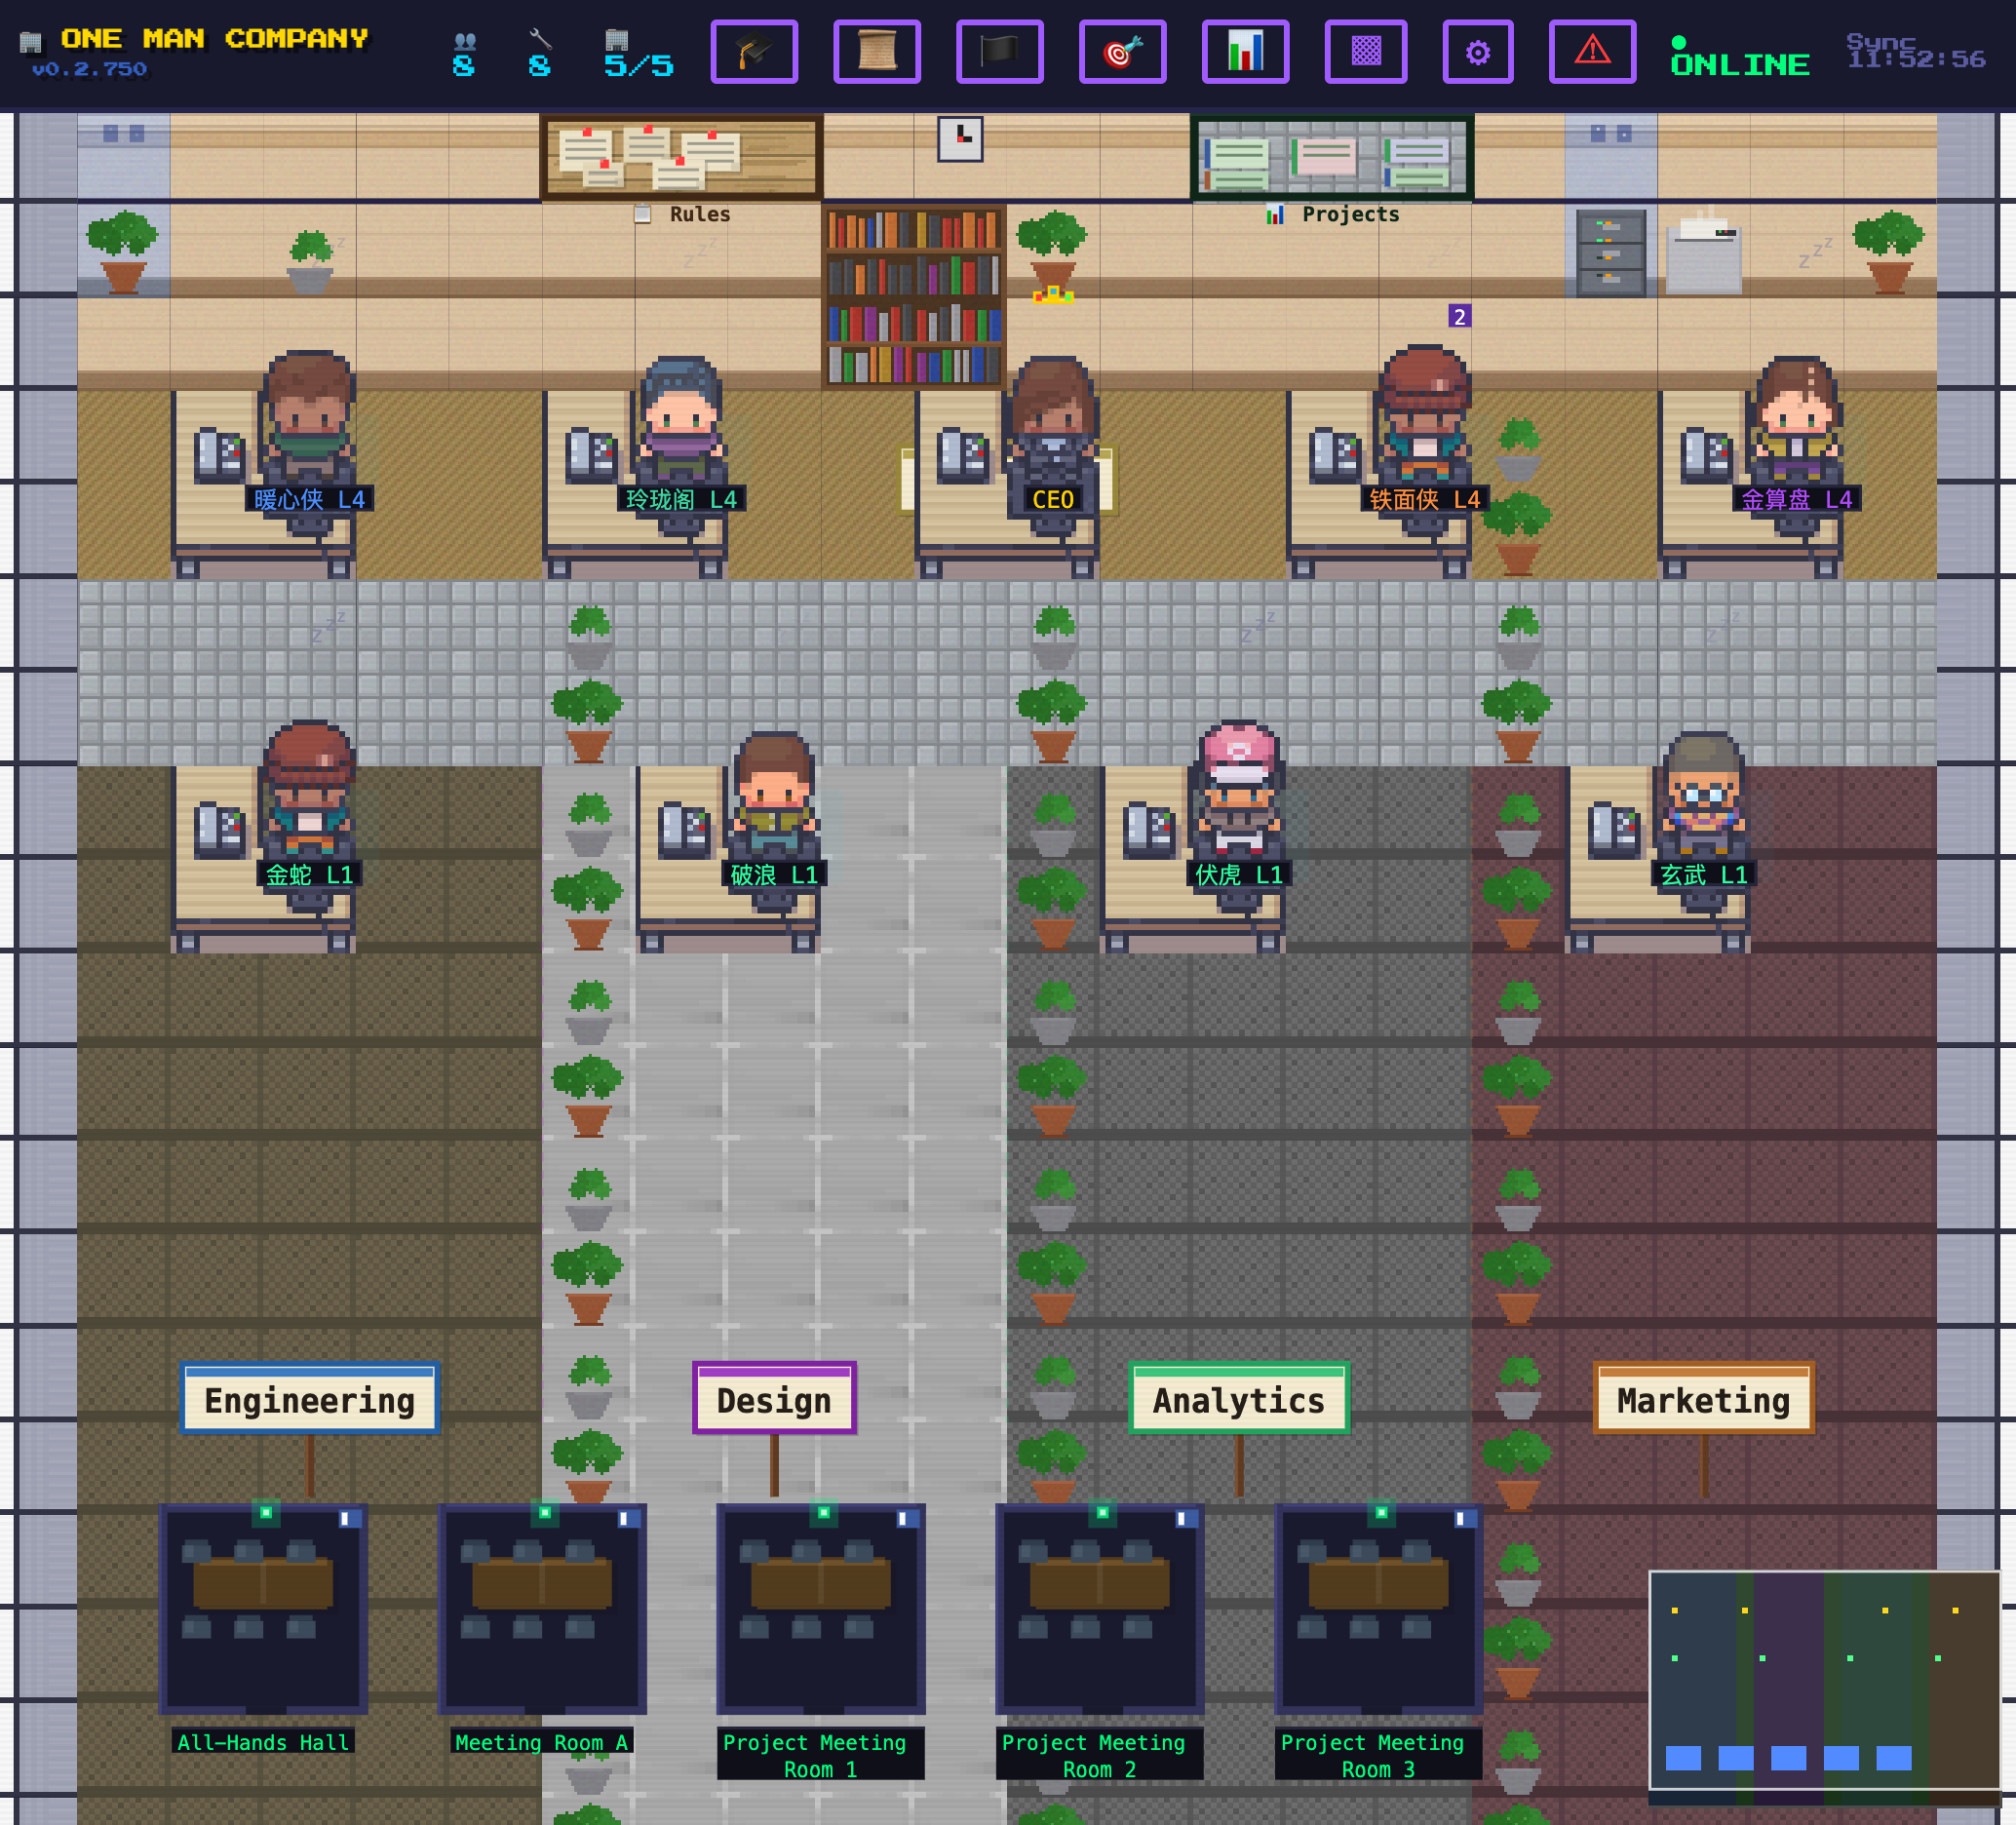
\includegraphics[width=\textwidth]{vide_1.png}\\
    \vspace{2pt}
    {\small(a) Assembled team workspace}
\end{minipage}
\hfill
\begin{minipage}[c]{0.30\textwidth}
    \centering
    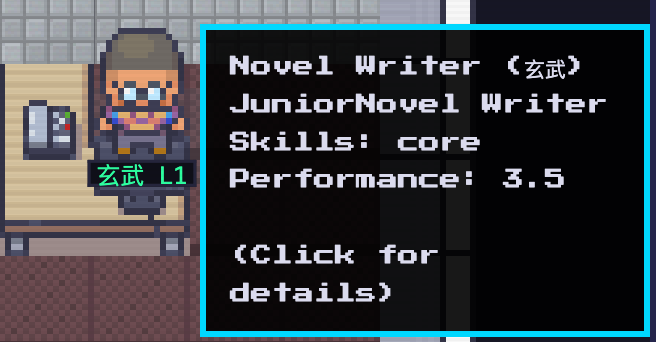
\includegraphics[width=\textwidth]{vide_2.png}\\
    \vspace{2pt}
    {\small(b) Novel Writer AI Agent}
    \vspace{6pt}
    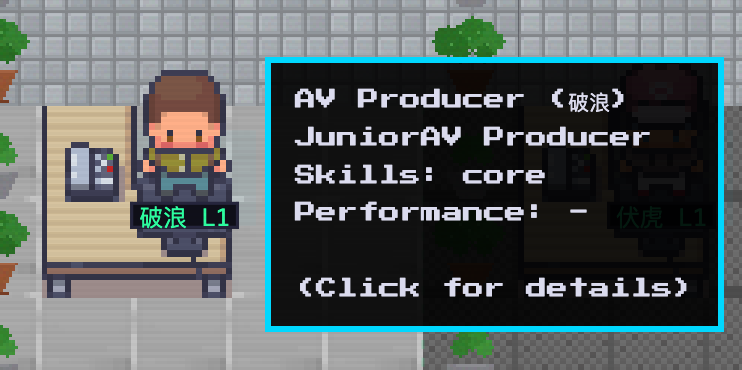
\includegraphics[width=\textwidth]{vide_3.png}\\
    \vspace{2pt}
    {\small(c) AV Producer AI Agent}
\end{minipage}
\hfill
\begin{minipage}[c]{0.30\textwidth}
    \centering
    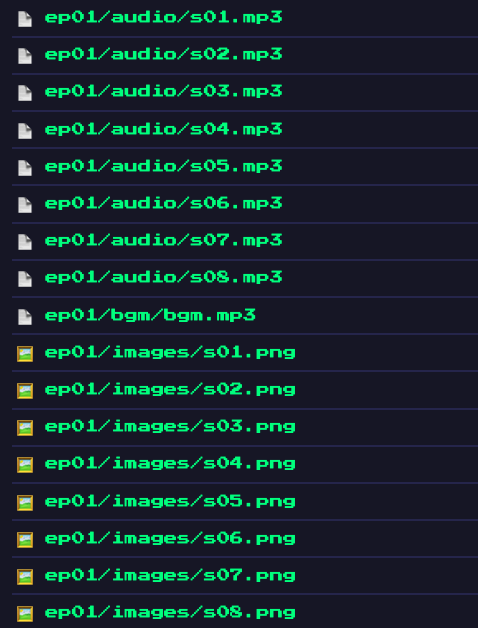
\includegraphics[width=\textwidth]{vide_4.png}\\
    \vspace{2pt}
    {\small(d) Project output artefacts}
    \vspace{6pt}
    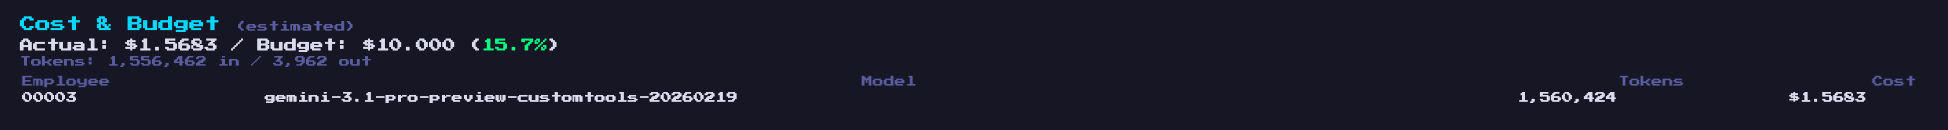
\includegraphics[width=\textwidth]{vide_5.png}\\
    \vspace{2pt}
    {\small(h) Cost \& token breakdown}
\end{minipage}
\caption{
    \textbf{AI short drama case study: team assembly, recruited agents, generated scenes, and cost breakdown.}
    (a)~Company workspace after team assembly.
    (b)--(c)~Profile cards of the two recruited Talents.
    (d)~Output artefacts including episode scripts, scene images, voice-over audio, and final videos.
    (h)~Cost breakdown: approximately 1.56M tokens at \$1.57 total (15.7\% of the \$10 budget).
}
\label{fig:case-drama-workflow}
\end{figure}

\newpage

\section{Case 4: Research Survey - Mind Map}
\label{sec:research-mindmap}

Figure~\ref{fig:research-mindmap} shows the mind map produced autonomously by OMC for the world models survey case study (Section~\ref{sec:case-content}).  The map covers six themes---Foundations, Model-Based RL, Video/Generative Models, Language-Conditioned World Models, Sim-to-Real Transfer, and Frontier Architectures---with approximately 70 nodes referencing 35+ papers from 2021--2026.

\begin{figure}[H]
    \centering
    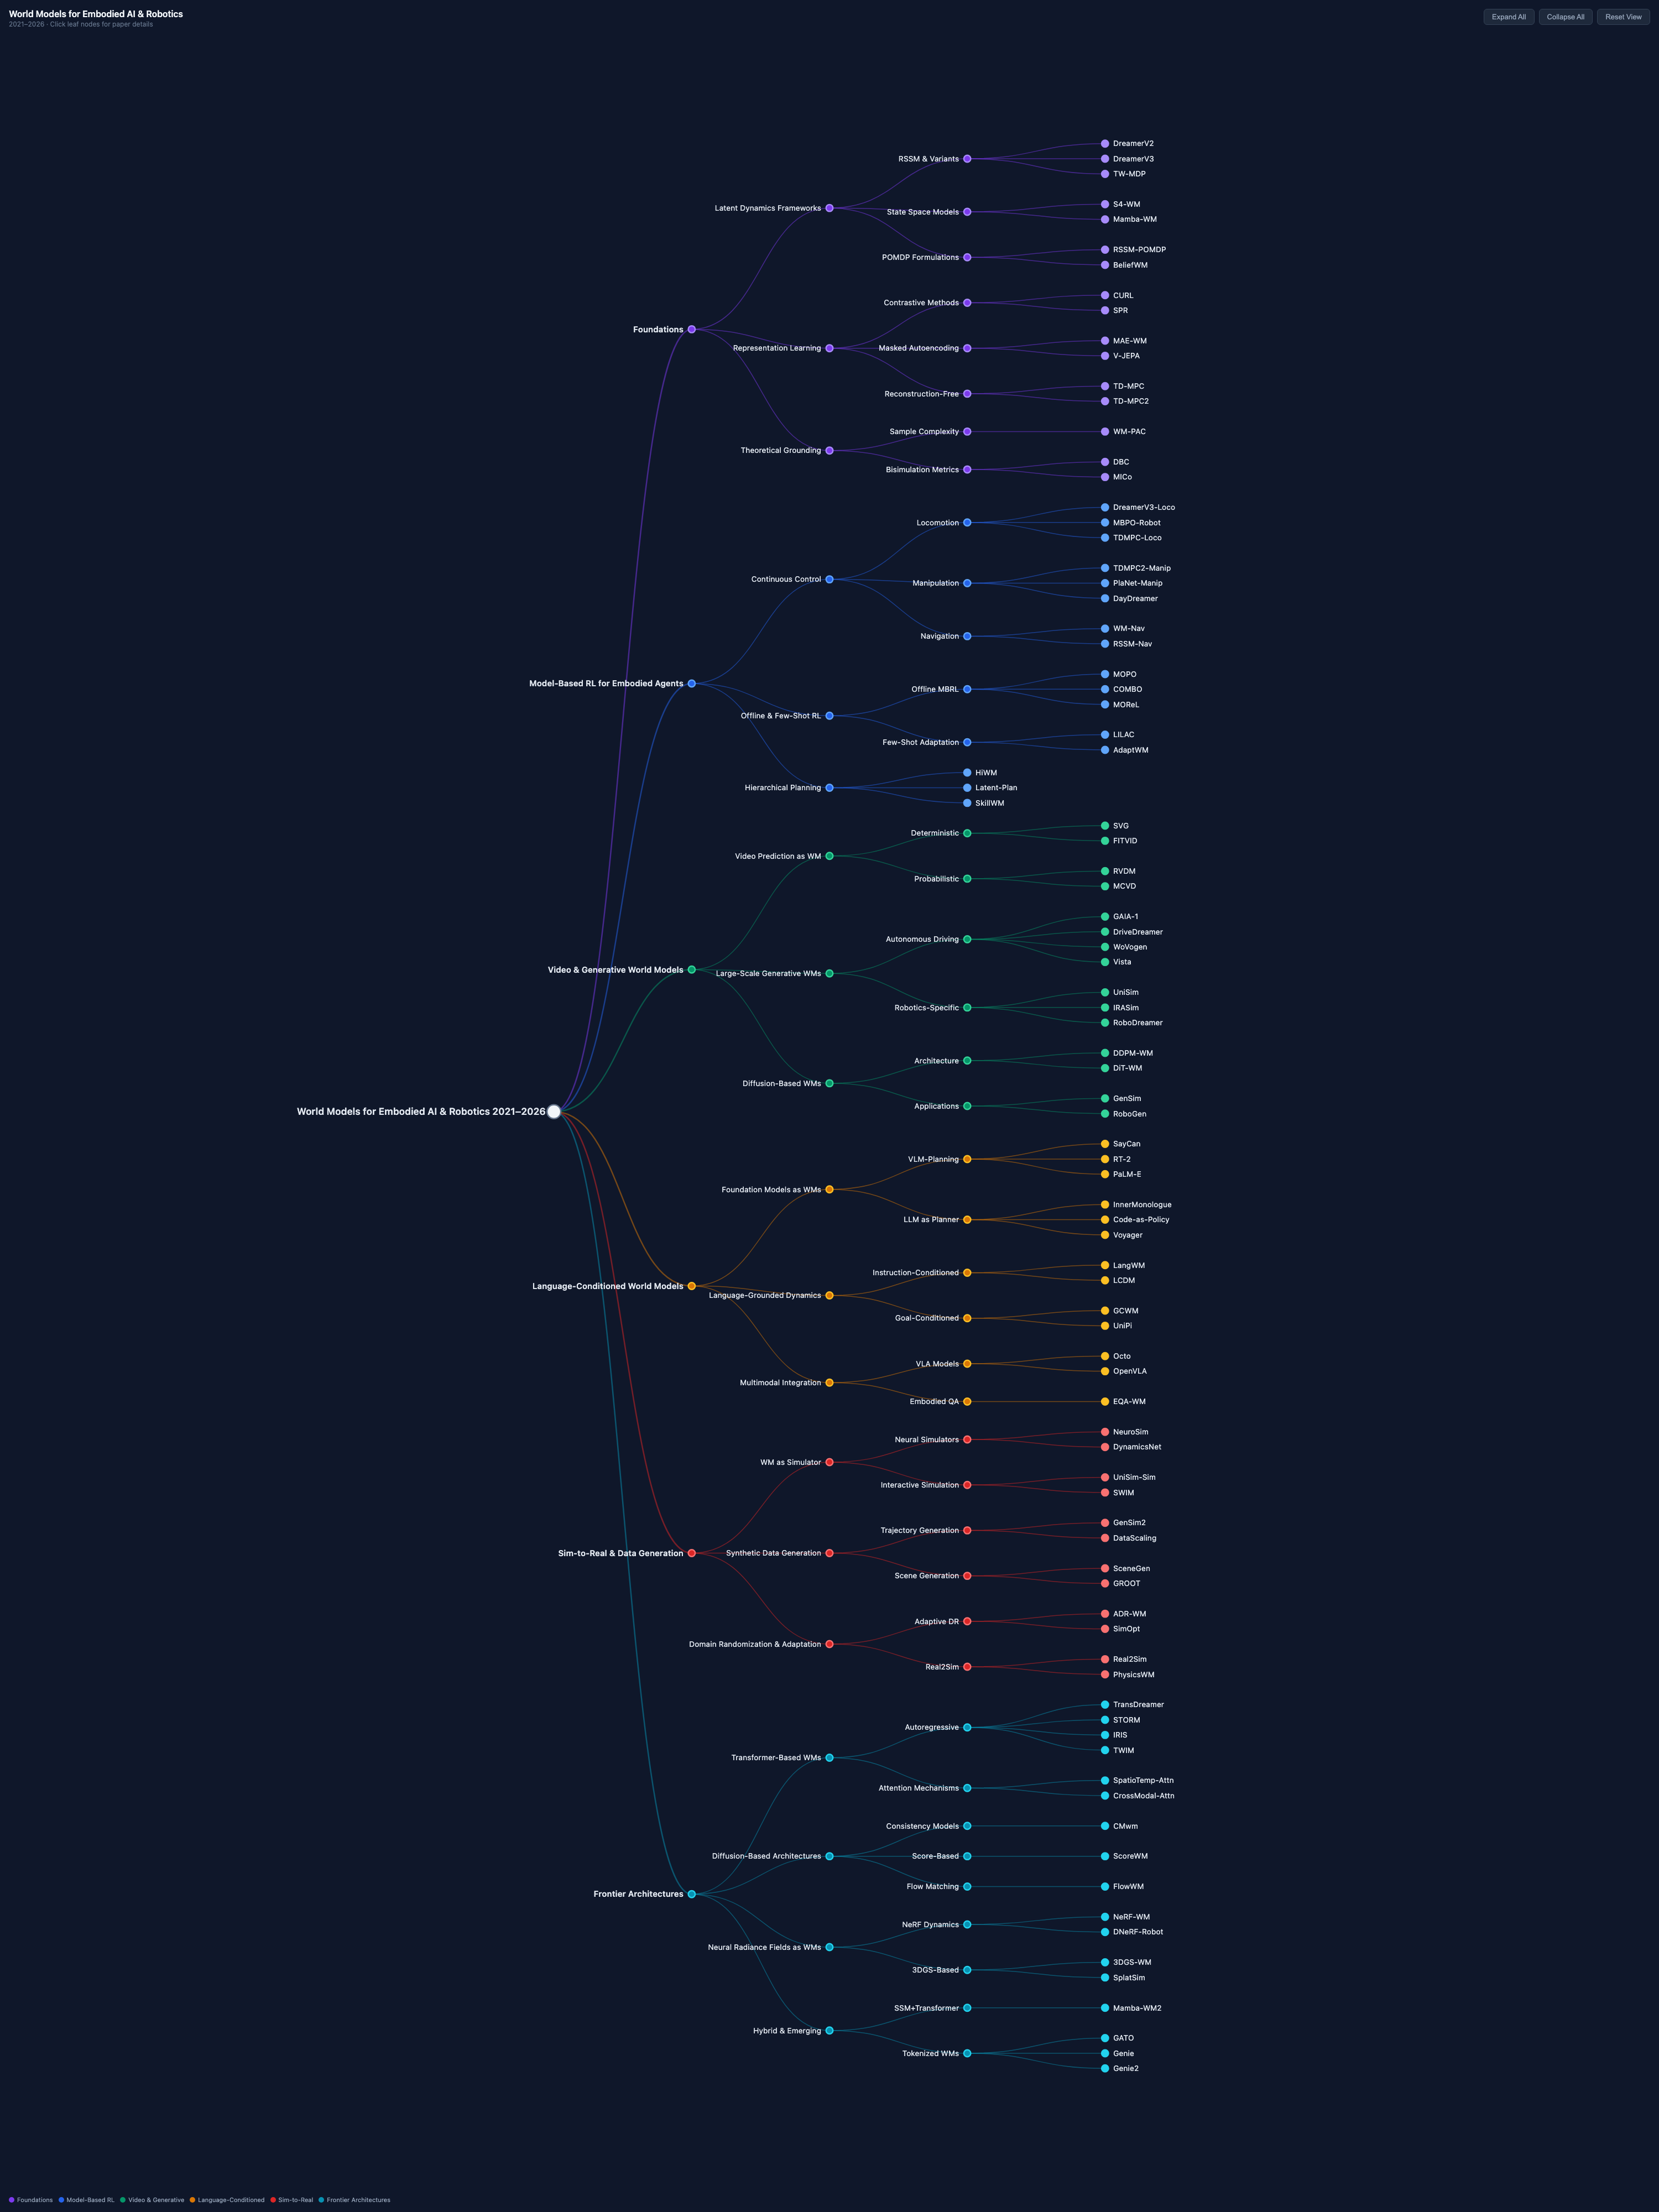
\includegraphics[width=0.9\textwidth]{case4/mindmap.png}
    \caption{Mind map generated autonomously by OMC's research team, covering six themes (Foundations, Model-Based RL, Video/Generative, Language-Conditioned, Sim-to-Real, Frontier Architectures) with approximately 70 nodes referencing 35+ papers from 2021--2026.}
    \label{fig:research-mindmap}
\end{figure}

\section{Case 4: Research Survey - Team and Generated Ideas}
\label{sec:research-ideas}

\begin{figure}[H]
\centering
%% Row 1: workspace + output documents
\begin{minipage}[c]{0.52\textwidth}
    \centering
    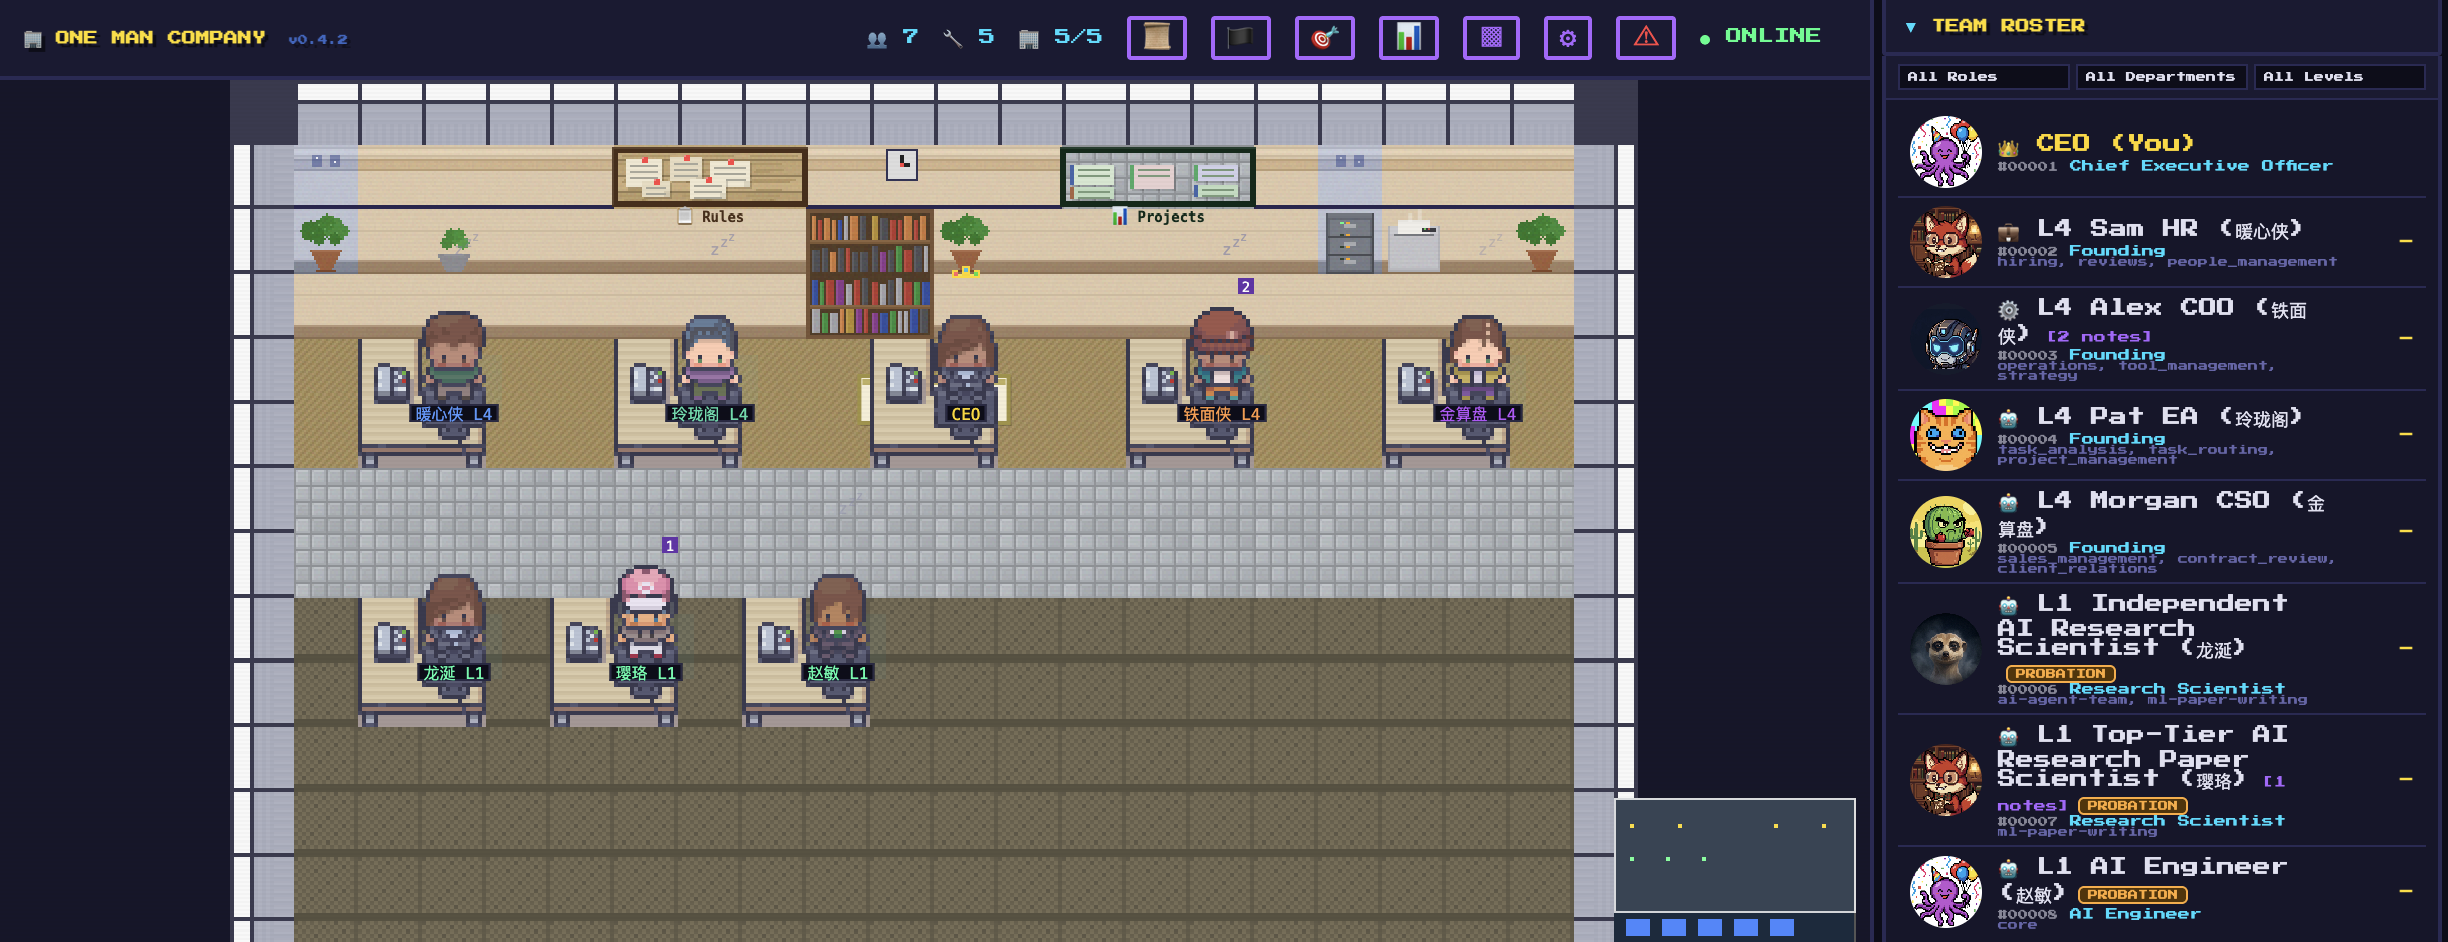
\includegraphics[width=\textwidth]{case4/all_agents.png}\\
    \vspace{2pt}
    {\small(a) Assembled research team}
\end{minipage}
\hfill
\begin{minipage}[c]{0.4\textwidth}
    \centering
    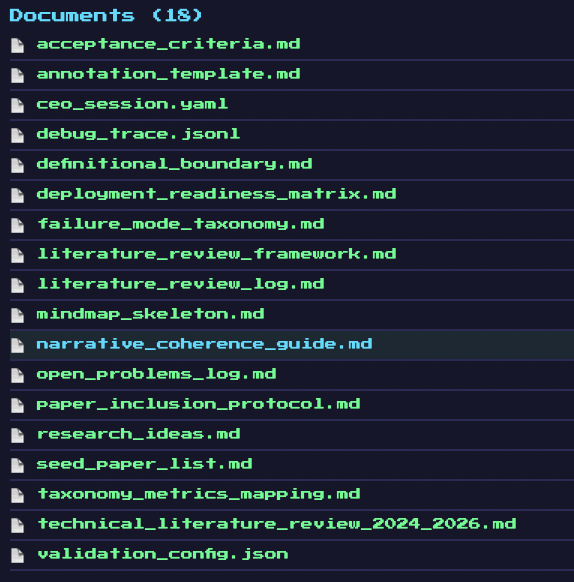
\includegraphics[width=\textwidth]{case4/filelist.png}\\
    \vspace{2pt}
    {\small(e) 17 output documents}
\end{minipage}

\vspace{8pt}

%% Row 2: agent profiles + cost
\begin{minipage}[c]{0.24\textwidth}
    \centering
    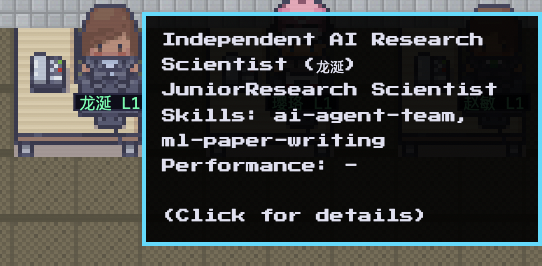
\includegraphics[width=\textwidth]{case4/reseascher_1.png}\\
    \vspace{2pt}
    {\small(b) Research Scientist}
\end{minipage}
\hfill
\begin{minipage}[c]{0.24\textwidth}
    \centering
    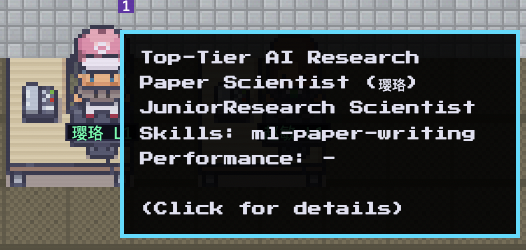
\includegraphics[width=\textwidth]{case4/reseascher_2.png}\\
    \vspace{2pt}
    {\small(c) Research Paper Scientist}
\end{minipage}
\hfill
\begin{minipage}[c]{0.24\textwidth}
    \centering
    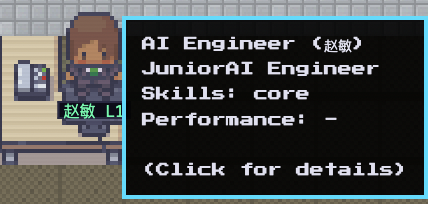
\includegraphics[width=\textwidth]{case4/engineer_1.png}\\
    \vspace{2pt}
    {\small(d) AI Engineer}
\end{minipage}
\hfill
\begin{minipage}[c]{0.24\textwidth}
    \centering
    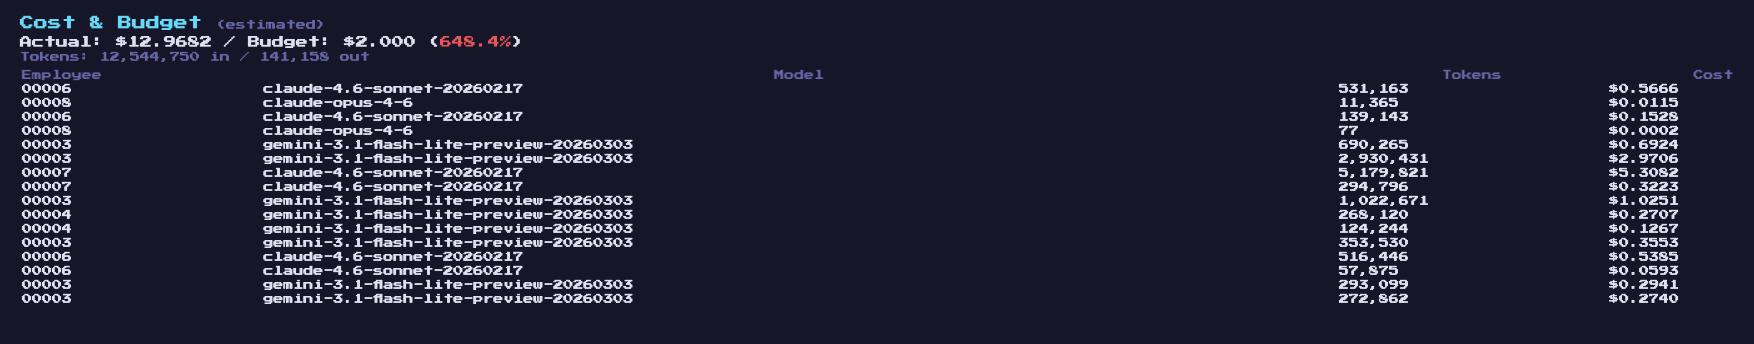
\includegraphics[width=\textwidth]{case4/cost.png}\\
    \vspace{2pt}
    {\small(f) Cost \& token breakdown}
\end{minipage}

\caption{
    \textbf{Automated research survey case study.}
    (a)~The OMC workspace after team assembly, with three recruited specialists seated alongside the founding team.
    (b)--(d)~Profile cards of the recruited Talents: two Research Scientists (Claude Sonnet~4.6) and one AI Engineer (self-hosted).
    (e)~The 18 deliverable documents produced autonomously, including literature reviews, failure mode taxonomies, and research proposals.
    (f)~Cost and token breakdown: \$16.26 total across 15.9M tokens.
}
\label{fig:case-research}
\end{figure}

The three research ideas below were generated autonomously by OMC's research team, grounded in the failure modes (FM) identified during the survey.  The FM codes refer to entries in the team's failure mode taxonomy: FM-001 (compounding prediction error), FM-002 (physical implausibility), FM-003 (sim-to-real domain shift), and FM-008 (overconfident hallucination).

\subsection*{Idea 1: HiTeWM (Hierarchical Temporal World Models)}
\textbf{Problem}: Compounding prediction error (FM-001)---DreamerV3 degrades beyond 15 steps; RoboDreamer achieves only 15\% success on long-horizon tasks.  \textbf{Approach}: Two-level architecture with a fast model (50 Hz, RSSM-style, $\sim$50M params) for short-horizon dynamics and a slow model (2 Hz, Transformer-based) for macro-state transitions.  An uncertainty-gated re-grounding mechanism injects real observations when ensemble disagreement exceeds a learned threshold, converting pure imagination into closed-loop prediction.  \textbf{Expected improvement}: 30--50\% on 100+ step tasks vs.\ DreamerV3.

\subsection*{Idea 2: PhysWM (Physics-Grounded Latent World Models)}
\textbf{Problem}: Physical implausibility (FM-002)---video-based world models generate trajectories that violate conservation laws and contact constraints.  \textbf{Approach}: A Physics Constraint Module injects differentiable physics priors (rigid-body dynamics, energy conservation) into the latent transition function as soft penalties.  \textbf{Expected improvement}: 40--60\% in physical plausibility score; 20--35\% on contact-rich manipulation tasks.

\subsection*{Idea 3: MAWM (Meta-Adaptive World Models)}
\textbf{Problem}: Sim-to-real domain shift (FM-003) compounded by overconfident hallucination (FM-008).  \textbf{Approach}: Meta-learning across randomised sim domains produces an initialisation that adapts with $K{=}5$ real trajectories.  Conformal prediction provides calibrated uncertainty bounds, preventing the planner from acting on hallucinated predictions.  \textbf{Expected improvement}: $>$80\% task success with $K{=}5$ vs.\ $\sim$50--65\% baseline.


\end{document}